%%%%%%%% ICML 2018 EXAMPLE LATEX SUBMISSION FILE %%%%%%%%%%%%%%%%%

\documentclass{article}

% Recommended, but optional, packages for figures and better typesetting:
\usepackage{microtype}
\usepackage{graphicx}
\usepackage{caption}
\usepackage{subcaption}
\usepackage{booktabs} % for professional tables

% hyperref makes hyperlinks in the resulting PDF.
% If your build breaks (sometimes temporarily if a hyperlink spans a page)
% please comment out the following usepackage line and replace
% \usepackage{icml2018} with \usepackage[nohyperref]{icml2018} above.
\usepackage[draft]{hyperref}

% Attempt to make hyperref and algorithmic work together better:
\newcommand{\theHalgorithm}{\arabic{algorithm}}

% show comments
\newcommand{\yitao}[1]{\textcolor{blue}{\textbf{[Yitao: #1]}}}


% Use the following line for the initial blind version submitted for review:
\usepackage{icml2018}
\usepackage{natbib}
\usepackage{amsmath}
\usepackage{amsthm}
\usepackage{amsfonts}
\usepackage{bbm}
\usepackage{bm}
\usepackage{amssymb}
\usepackage{enumitem}
\newtheorem{theorem}{Theorem}
\newtheorem{proposition}[theorem]{Proposition}
\theoremstyle{lemmas}
\newcounter{lemmas}
\newtheorem{lemma}[lemmas]{Lemma}
\newtheorem{definition}{Definition}
\makeatletter
\renewenvironment{proof}[1][\proofname]{\par
  \vspace{-\topsep}% remove the space after the theorem
  \pushQED{\qed}%
  \normalfont
  \topsep0pt \partopsep0pt % no space before
  \trivlist
  \item[\hskip\labelsep
        \itshape
    #1\@addpunct{.}]\ignorespaces
}{%
  \popQED\endtrivlist\@endpefalse
  \addvspace{0pt plus 0pt} % some space after
}
\makeatother

\ifodd 1
\newcommand{\rev}[1]{{\color{blue}#1}}%revise of the text
\newcommand{\com}[1]{\textbf{\color{red}(Yang: #1)}} %comment of the text
\newcommand{\clar}[1]{\textbf{\color{green}(NEED CLARIFICATION: #1)}}
\newcommand{\response}[1]{\textbf{\color{magenta}(RESPONSE: #1)}} %response to comment
\else
\newcommand{\rev}[1]{#1}
\newcommand{\com}[1]{}
\newcommand{\clar}[1]{}
\newcommand{\response}[1]{}
\fi

% Supplementary File
\usepackage{xr-hyper}
\externaldocument[Su-]{Supplementary}

% If accepted, instead use the following line for the camera-ready submission:
%\usepackage[accepted]{icml2018}

% The \icmltitle you define below is probably too long as a header.
% Therefore, a short form for the running title is supplied here:
\icmltitlerunning{Inference Aided Reinforcement Learning for Incentive Mechanism Design in Crowdsourcing}

\begin{document}

\twocolumn[
%\icmltitle{Incentive Compatible Reinforcement Bayesian Inference for Crowdsourcing}
\icmltitle{Inference Aided Reinforcement Learning for\\Incentive Mechanism Design in Crowdsourcing}

% It is OKAY to include author information, even for blind
% submissions: the style file will automatically remove it for you
% unless you've provided the [accepted] option to the icml2018
% package.

% List of affiliations: The first argument should be a (short)
% identifier you will use later to specify author affiliations
% Academic affiliations should list Department, University, City, Region, Country
% Industry affiliations should list Company, City, Region, Country

% You can specify symbols, otherwise they are numbered in order.
% Ideally, you should not use this facility. Affiliations will be numbered
% in order of appearance and this is the preferred way.
\icmlsetsymbol{equal}{*}

\begin{icmlauthorlist}
\icmlauthor{Zehong Hu}{NTU}
\icmlauthor{Yitao Liang}{UCLA}
\icmlauthor{Yang Liu}{Harvard}
\icmlauthor{Jie Zhang}{NTU}

\icmlaffiliation{NTU}{Rolls-Royce Cooperate Lab@NTU, School of Computer Science and Engineering, Nanyang Technological University, Singapore}
\icmlaffiliation{UCLA}{Computer Science Department, University of California, USA}
\icmlaffiliation{Harvard}{Computer Science Department, Harvard University, USA}
\end{icmlauthorlist}

%\icmlaffiliation{goo}{Googol ShallowMind, New London, Michigan, USA}
%\icmlaffiliation{ed}{School of Computation, University of Edenborrow, Edenborrow, United Kingdom}
%\icmlcorrespondingauthor{Cieua Vvvvv}{c.vvvvv@googol.com}
%\icmlcorrespondingauthor{Eee Pppp}{ep@eden.co.uk}

% You may provide any keywords that you
% find helpful for describing your paper; these are used to populate
% the "keywords" metadata in the PDF but will not be shown in the document
\icmlkeywords{crowdsourcing, reinforcement learning, mechanism design}

\vskip 0.3in
]

\begin{abstract}
%In crowdsourcing, incentive mechanisms are designed to incentivize workers to report high-quality labels.
%However, existing mechanisms are often developed as one-shot static solutions, assuming that the designer knows how worker respond to certain incentive levels in exerting effort, and that all workers follow certain utility-maximizing strategy.
%In this paper, we build a sequential data acquisition mechanism that leverages the power of reinforcement learning. We firstly develop a Bayesian inference algorithm to estimate workers' states by fully exploiting all the collected labels.
%Then, we propose a reinforcement learning algorithm, relying on the above state estimation, to uncover how workers respond to the different offered incentive levels, and how workers' states (accuracy in contributed labels) changes. %mine the connection between workers' state changes and the incentives.
%Our mechanism determines the incentives for workers based on the estimates of workers' states and the output of the reinforcement learning algorithm.
%We theoretically prove that our mechanism correctly incentivizes workers to report high-quality labels.
%Besides, the empirical results show that our Bayesian inference algorithm can improve the robustness and lower the variance of incentives, and our mechanism performs consistently well when different kinds of workers are tested.

In crowdsourcing, incentive mechanisms are designed to incentivize self-interested workers to report high-quality labels.
However, existing mechanisms are often developed as one-shot static solutions, assuming that all workers follow the utility-maximizing strategy.
In this paper, we build a sequential data acquisition mechanism by firstly developing a Bayesian inference algorithm to estimate workers' labeling strategies from the collected labels.
Then, we propose a reinforcement learning algorithm, relying on the above estimates, to uncover how workers respond to the incentives. Our mechanism determines the incentives for workers based on workers' current strategies and the output of the reinforcement learning algorithm.
We theoretically prove that our mechanism can correctly incentivize workers to provide high-quality labels.
We also empirically show that our Bayesian inference algorithm can improve the robustness and lower the variance of incentives, and our mechanism performs consistently well when different kinds of workers are tested.
\end{abstract}



\section{Introduction}
The ability to quickly collect large scale and high quality labeled datasets is crucial for Machine Learning, and more generally Artificial Intelligence. Among all proposed solutions, one of the most promising ones is crowdsourcing \cite{} [cite AMT, imagenet]. The idea is neat - instead of using a centralized amount of efforts, the labeling tasks will be disseminated to a decentralized crowd of workers, leveraging the power of human computation, to parallelize this collection procedure. Nonetheless, it has been noted not after a long time of this proposal that, crowdsourced data often suffered from quality issues, due to its unique feature of no monitoring and no ground-truth verification of workers' contributed data. 

The above quality control challenge has been attempted to resolve by two rather disconnected research communities separately. From the more Machine Learning side, a family of variational and Bayesian inference techniques developed for inferring true labels from crowdsourced and potentially noisy labels \cite{}, often working as a one-shot, post-processing procedure facing a static set of workers, whose labeling accuracy is fixed and \emph{informative}. Despite its nice theoretical contribution and empirical success, the above methods ignored the effects of \emph{incentives} when dealing with human inputs. It has been observed both in theory and practice that \cite{}, without appropriate incentive, selfish and rational workers can easily chose to contribute low quality, uninformative, or even malicious data. Existing inferences are very vulnerable in these cases - either much more redundant crowdsourced labels will need to be collected (low quality inputs), or the methods will simply fail to work (the case with uninformative and malicious inputs). 

The above data quality control question has been studied in the context of \emph{incentive design}, mostly in a non-ML setting (except for \cite{cite my EC'17 paper}). In particular, a family of mechanisms, jointly called \emph{peer prediction}, has been proposed towards addressing above incentive challenges \cite{}. Existing peer prediction mechanisms focus on achieving incentive compatibility (IC) defined as the reporting a high quality data will maximizes the expected payment issued to workers. The idea is to achieve IC via comparing the reports between the targeted reported data, and a randomly selected reference answer. We note several undesirable properties of peer prediction, which we suspect are the reasons that lead to its inconsistent performance in practice \cite{}. First, existing peer prediction mechanisms simplify workers' responses to the incentive mechanism by assuming that workers are all fully rational and only follow the utility-maximizing strategy. However, there is evidence showing that human workers are not always fully rational, and they may deviate from equilibrium strategies. Thus, these peer prediction mechanisms that are fancy in theory may yet fail in practice \cite{}. Secondly, existing mechanisms are not prior-free, meaning that workers' cost in exerting effort to produce high quality data is assumed to be known - this is unlikely to be the case in practice. Thirdly, we find that some other properties of incentives, such as variance of payment, robustness to the environments etc, are often overlooked, as well as the variation of incentives among different types of agents - we suspect partly this is because the existing methods only use a small amount of all collected labels.



We believe the above disconnection is far from being satisfactory and unnecessary. In this paper, we propose an incentive compatible \emph{reinforcement Bayesian inference} approach, aiming to marry and extend the above two areas and techniques, and to address the existing caveats in above incentive design and inference learning methods in a sequential setting. We chose to go with a sequentially interactive setting, not only because this is often the case in practice, but also we find this setting is extremely suitable for us to leverage reinforcement learning type of sequential learning algorithm to relax our algorithm to an entirely parameter- and model-free setting. 

The high level idea is as follows: at each step, we will leverage the power of Bayesian inference method to design an incentive mechanism to induce high effort from workers. Driving in the background, we develop a reinforcement learning algorithm to sequentially interact with agents to learn their best incentive levels. 

Addressing above challenges are not technically easy. There is a line of challenges that need to be addressed. We list several key ones here:
\begin{itemize}
\item In order to achieve good incentive property and calibrate the accuracy workers' reported information, there is a need of having an unbiased inference algorithm. Unfortunately this is not the case with existing inference method. %Also we need to prove the convergence of such an inference algorithm. 
\item In order to learn the right incentive for each agent, we will leverage reinforcement learning as the underlying sequentially interactive algorithm. Nonetheless
\begin{itemize}
\item The state of RL is missing: due to unobservable workers' work state;
\item The reward state, i.e., how well workers respond to each level of offered payment is unbservable: this is again due to no ground-truth, as well as the unobservability of workers' state.
\item Possibility of long term manipulation: agents can hope to contribute malicious data in hope of a long term return. 
\end{itemize}
\end{itemize}


We summarize two core contributions in this paper:
\begin{itemize}
\item We propose a novel one-shot peer prediction mechanism based on Bayesian inference. Since existing Bayesian inference algorithms (e.g. EM estimator and variational inference) for crowdsourcing are biased in principle, we derive the explicit posterior distribution of the true labels and employ Gibbs sampling for inference. The most challenging problem of our mechanism is to prove the convergence of above inference method, and further the incentive compatibility of our mechanism which has never been explored in the literature. 

We prove our method can calibrate the accuracy of each agent's reported works, and thus provides strong incentives for workers to exert effort and report truthfully their data. Among all advantages, we note that our method is robust to the existence of low quality but highly correlating signals (e.g., essay length in the peer grading case). Besides, we also empirically show the advantages of our mechanism on the stability and fairness of incentives over existing ones.
\item We design the first reinforcement Bayesian inference framework which sequentially interacts with workers, addressing the issues of unobservable states and rewards. It dynamically adjusts the scaling level of our incentive mechanism to maximize the utility of the data requester, as well as to estimate the true states and rewards for each corresponding actions. To avoid assuming a decision-making model for workers, we use the data-driven Gaussian process to represent the scaling level adjustment policy, and online updates our policy according to workers' responses. 

We prove a sufficient condition under which the reinforcement learning algorithm we built is robust to long term manipulation of each agent too. Thus we are able to avoid the case where agents are not greedy (or often referred to as simple agents in the literature) and are strategic in reasoning long term returns. This robust to manipulation result only shows the benefits of our reinforcement learning algorithm. We also empirically show its advantages on improving the utility if the data requester over one-shot mechanisms.
\end{itemize}

The rest of the paper organizes as follows: XXXX.
\section{Related Work}
There have been a few pioneering studies which improves incentive mechanisms by incorporating machine learning techniques.
For example, to improve the long-term utility of the data requester in crowdsourcing, \citet{liu2017sequential} develop a multi-armed bandit algorithm to adjust the state-of-the-art peer prediction mechanism, DG13~\cite{dasgupta2013crowdsourced}.
However, both the bandit algorithm and DG13 still need to assume that workers are fully rational and will behave as we desired.
Instead of randomly choosing a reference worker, \citet{liu2017machine} propose to use supervised learning algorithms to generate the reference reports based on the contextual information of tasks and derive the incentive compatibility conditions for the supervised-learning-based peer prediction mechanisms.
In this paper, without assuming the contextual information about tasks, we develop an unsupervised-learning algorithm to learn the worker models and true labels from.
Our payments are determined based on the learned worker models, and we derive the incentive compatibility conditions for our unsupervised-learning-based mechanism.
Besides, in e-commerce, to be adapted to different kind of agents, \citet{RMDE,cai2018reinforcement} propose to build incentive mechanisms based on reinforcement learning.
However, focusing on the empirical analysis, they never consider the theoretical incentive compatibility.
In this paper, we also incorporate reinforcement learning to get rid of the assumption that workers are fully rational.
When analyzing our incentive mechanism, we go one-step further by not only providing the empirical analysis but also present a novel proof for the incentive compatibility related with reinforcement learning.


%Peer prediction \cite{Prelec:2004,MRZ:2005,jurca2006minimum,jurca2009mechanisms,witkowski2012robust,witkowski2012peer,radanovic2013,dasgupta2013crowdsourced}, a class of mechanisms that have been developed extensively recently, are often adopted for incentivizing truthful or high-quality contributions from strategic sources when the quality of the contributions cannot be verified. %The Bayesian Truth Serum was proposed in \cite{Prelec:2004} to elicit truthful report when only minority of the crowd holds the true answer. 
%Particularly, the seminal work \cite{MRZ:2005} established that strictly proper scoring rule \cite{Gneiting:07} can be adopted in the peer prediction setting for eliciting truthful reports; following which a sequence of followed up works have been done on relaxing the assumptions that have been imposed therein \cite{witkowski2012robust,witkowski2012peer,radanovic2013}. More recently, \cite{Witkowski_hcomp13,dasgupta2013crowdsourced} formally introduced and studied an effort sensitive model for binary signal data elicitation. Particularly \cite{dasgupta2013crowdsourced} proposed a multi-task peer prediction mechanism that can help remove undesirable equilibria that lead to low quality reports. These results are further strengthened and extended to a non-binary signal setting in \cite{2016arXiv160303151S,kong2016framework}. One set of studies focuses on using models that aggregate tasks from different agents \cite{kamar2012incentives,faltings2014incentive,radanovic2016incentives}. These work do not consider a machine learning setting, and have not established a rigorous analysis. 
%
%
%
%[add inference and reinforcement learning]
\section{Problem Formulation}
\label{PF}
This paper focuses on typical crowdsourcing problems. To be more specific, at each time step $t$, one data requester assigns $M$ tasks with binary answer space $\left\{1,2\right\}$ to $N \geq 3$ candidate workers to label. Workers receive payments for finishing the labeling tasks. We use $L^t_i(j)$ to denote the label worker $i$ generates for task $j$ at time $t$. For simplicity of computation, we reserve $L^t_i(j) = 0$ if  $j$ is not assigned to $i$. Furthermore, we use $\mathcal{L}$ and $\bm{L}$ to denote the set of ground-truth labels and  the set of all collected labels respectively.

%The generated label $L^{t}_{i}(j)$ depends both on the ground-truth label $L^{t}(j)$ and worker $i$'s effort level $e^{t}_i$ and reporting strategy $r^{t}_i$.
%Any worker $i$ can potentially have two effort levels, High ($e^{t}_i=1$) and Low ($e^{t}_i=0$).
%Also, he/she can decide either to truthfully report his observation $r^{t}_i = 1$ or to revert the answer $r^{t}_i = 0$.
%Workers may act differently for different tasks. 
%We thus define $e^{t}_i\in[0,1]$ and $r^{t}_i\in[0,1]$ as worker $i$'s probability of exerting high efforts and being truthful, respectively.
%In this case, worker $i$'s probability of being correct (PoBC) can be computed as
%\begin{equation}
%\begin{split}
%&p^{t}_i=r^{t}_i e^{t}_i p_{i, H}+r^{t}_i (1-e^{t}_i) p_{i, L}+\\
%&(1-r^{t}_i) e^{t}_i (1-p_{i, H})+(1-r^{t}_i) (1-e^{t}_i) (1-p_{i, L})
%\end{split}
%\end{equation}
%where $p_{i, H}$ and $p_{i, L}$ denote worker $i$'s probability of observing the correct label when exerting high and low efforts, respectively.
%Following \cite{dasgupta2013crowdsourced,liu2017sequential}, we assume that the tasks are homogeneous and the workers share the same set of $p_{i, H}, p_{i, L}$, denoting by $p_H, p_L$, and $p_{H}>p_{L}= 0.5$.
%Here, $p^t_i=0.5$ means that worker $i$ randomly selects a label to report.

The generated label $L^{t}_{i}(j)$ depends both on the ground-truth $\mathcal{L}(j)$ and worker $i$'s strategy, which is mainly determined by two factors, effort level (high or low) and reporting strategy (truthful or deceitful).
Accommodating the notation commonly used in reinforcement learning, we also refer worker i's strategy as his/her internal state.
%Any worker $i$ can potentially have two effort levels, High ($e^{t}_i=1$) and Low ($e^{t}_i=0$).
%Also, he/she can decide either to truthfully report his observation $r^{t}_i = 1$ or to revert the answer $r^{t}_i = 0$.
%Workers may act differently for different tasks. 
At any given time for any task, workers at their will adopt an arbitrary combination of effort level and report strategy. We thus define $\textsf{eft}^{t}_i\in[0,1]$ and $\textsf{rpt}^{t}_i\in[0,1]$ as worker $i$'s probability of exerting high efforts and reporting truthfully for task $j$ %at time $t$ 
respectively. Furthermore, following existing literature \cite{dasgupta2013crowdsourced,liu2017sequential}, we assume that tasks are homogeneous and workers share the same probability of generating the correct labels if they exert the same level of efforts. We denote the probability as $\mathbb{P}_{H}$ and $\mathbb{P}_{L}$ respectively. Note we require $\mathbb{P}_{H} > \mathbb{P}_{L} = 0.5$. Besides, we further assume the cost for any worker $i$ to exert low effort is $c_{L} = 0$, whereas exerting high effort incurs $c_{H} \geq 0$.\footnote{We make such assumption for simplicity. Our analysis can be extended to the case where both $c_{L},  c_{H} \geq 0$, as long as $c_{H} \geq c_{L}$.}
Worker $i$'s probability of being correct (PoBC) at time $t$ for any given task is then given by
\begin{equation}
\label{PPP}
\begin{split}
&\mathbb{P}^{t}_i  = ~\textsf{rpt}^{t}_i \cdot\textsf{eft}^{t}_i \mathbb{P}_{H}+ (1-\textsf{rpt}^{t}_i)\cdot \textsf{eft}^{t}_i (1-\mathbb{P}_{ H})+\\
&\textsf{rpt}^{t}_i \cdot(1-\textsf{eft}^{t}_i) \mathbb{P}_{L}+(1-\textsf{rpt}^{t}_i) \cdot(1-\textsf{eft}^{t}_i) (1-\mathbb{P}_{L})
\end{split}
\end{equation}
Suppose we assign $m^{t}_i\leq M$ tasks to worker $i$ at time step $t$, then his or her utility would be 
\begin{equation}
\label{equation:u_of_worker}
u_i^t={\sum}_{j=1}^{M}P_i^t(j) - m^{t}_i \cdot c_H\cdot \textsf{eft}^{t}_i
\end{equation}
where $P^{t}_{i}$ denotes our payment to worker $i$ for task $j$ at time $t$ (see Section~\ref{payment} for more details).

%Suppose we assign $m^{t}_i$ tasks to worker $i$ at $t$, his utility is 
%\begin{equation}
%u_i^t=P_i^t - m^{t}_i \cdot c_H (\mathbb{P}_i^t-0.5)
%\end{equation}
%where $P^{t}_{i}$ denotes our payment to worker $i$ at step $t$ (see Section~\ref{payment} for details).
 
At the beginning of each step, the data requester and workers mutually agree to a certain rule of payment determination, which would not be changed until the next time step.
%the data requester promises the workers a certain rule of payment determination which acts the contract between two sides and cannot be changed until the next time step.
The workers are self-interested and may change their strategies according to the expected utility $\mathbb{E}u_i^t$ he/she can get. It is not surprising that workers' different strategies would lead to different PoBCs and then different qualities of labels. After collecting the generated labels, it is a common procedure for the data requester to infer true labels $\tilde{L}^t(j)$ by running some inference algorithm.
%Please refer to \citet{zheng2017truth} for a good survey of the existing inference algorithms.
%Denote the the inferred true label of task $j$ by $\tilde{L}^{t}(j)$.
The aggregate label accuracy $A^t$ and the data requester's utility $r_t$ satisfy
\begin{equation}
\label{equation:utility}
\begin{split}
A^t&=\frac{1}{M}{\sum}_{j=1}^{M}1\left[\tilde{L}^{t}(j)=\mathcal{L}(j)\right]\\
r_t &= F(A^t) - \eta {\sum}_{i=1}^{N}{\sum}_{j=1}^{M}P^t_i(j)
\end{split}
\end{equation}
where $F(\cdot)$ is a non-decreasing monotonic function mapping accuracy to utility and $\eta>0$ is a tunable parameter balancing label quality and costs. Naturally, $F(\cdot)$ function is non-deceasing as higher accuracy is preferred.\footnote{We use $r$ to denote the data requester's utility as it is used as the reward in our RL algorithm. See Section 4.3 for details.} 

%Due to the sequential nature of our assignment problem, we introduce the cumulative utility $U(t)$ of the data requester from the current step $t$ as
%\begin{equation}
%U^t={\sum}_{k=1}^{\infty}\gamma^{k}u^{t+k}
%\end{equation}
%where $0\leq \gamma< 1$ is the discount rate for future utilities.
%The objective of our study is to maximize $U^t$ by optimally designing % the payment rule and the ex-post adjustment algorithm of the payment rule, which we call as 
%the incentive mechanism.

\begin{figure}[t]
 	\centering
	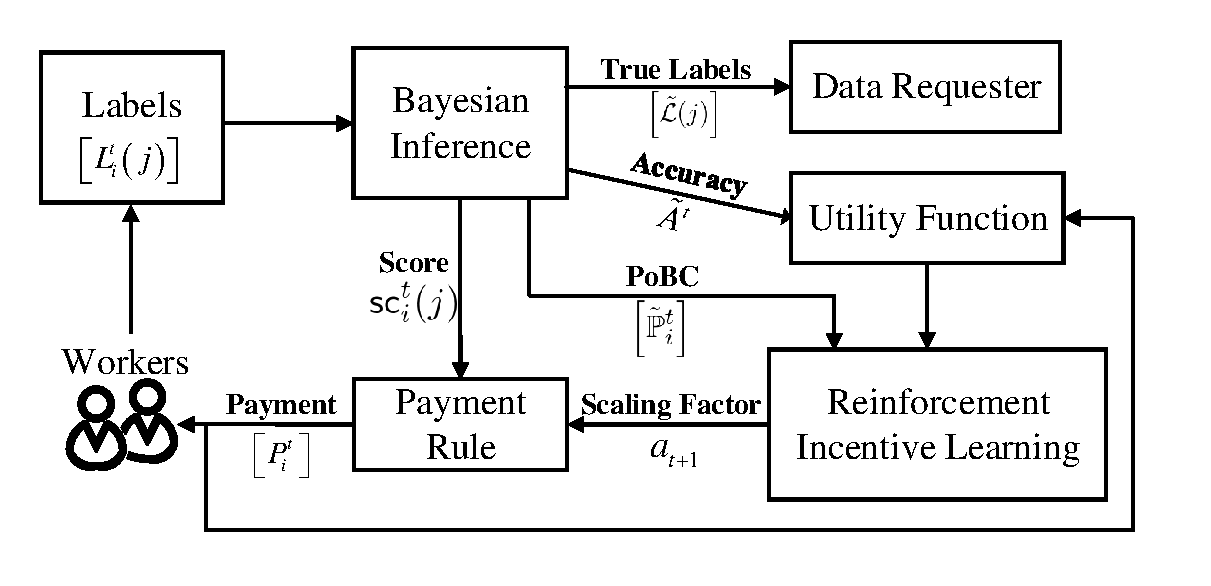
\includegraphics[width=0.48\textwidth]{image/Architecture}
	\vspace*{-8mm}
    \caption{\label{figure:layout} Layout of our incentive mechanism.}
\end{figure}
\section{Incentive Mechanism for Crowdsourcing}
We present the overall layout of our mechanism in Figure~\ref{figure:layout}, where estimated values are denoted with over-the-head tildes. In our design, the payment rule is to ensure that reporting truthfully and exerting high efforts  is the payment-maximizing strategy for all workers at any given time. Besides, our incentive mechanism as a whole guarantees that this is also the payment-maximizing strategy for all workers in the long run. We kindly refer readers to Section~\ref{analysis} for the theoretical proof. This property prevents strategic manipulations from workers, which bring more long-term benefits to them by sacrificing short-term ones, or the other way around. 
By doing so, we wish to induce workers to generate high-quality labels. %and thus improve the label accuracy. 
The Bayesian inference algorithm is responsible for estimating the true labels, workers' PoBCs and the aggregate label accuracy from the collected labels at each time step. It utilizes soft Dirichlet priors and Gibbs sampling to prevent overestimation of accuracy when workers generate poor-quality labels. The reinforcement learning algorithm adjusts the payment rule based on the historical data of payments, workers' PoBCs and aggregate labels' accuracy, aiming to optimally balance the utility gain from high accuracy and loss from large payments, which corresponds to $F(A^t)$ and $\sum_{i}P_i^t$ in Eqn.\ref{equation:utility} respectively.

In the rest of this section, we formally introduce the three main components of our design: payment rule, bayesian inference and reinforcement learning.

%Nevertheless, there are three challenges to achieve our design. Firstly, our empirical studies reveal that popular inference algorithms may be heavily biased towards overestimating the accuracy when the quality of labels is very low. For example, when there are $10$ workers and $q_i^t=0.55$, the estimated label accuracy of the EM estimator~\cite{dawid1979maximum,raykar2010learning} stays at around $0.9$ while the real accuracy is only around $0.5$.
%This heavy bias will cause the utility to be miscalculated and thus mislead our reinforcement adjustment.
%To reduce the inference bias, we develop our Bayesian inference algorithm by introducing the soft Dirichlet priors to both the true labels and workers' PoBCs.
%In this case, the posterior distribution cannot be expressed as any known distributions, which motivates us to derive the explicit posterior distribution at first and then employ Gibbs sampling to conduct inference.
%{\color{red}Secondly, the reinforcement adjustment expects the utility to be accurately calculated so that the direction of adjustment is clear.
%However, both the label accuracy and workers' PoBCs in our incentive mechanism are corrupted by noise.
%Considering that these estimates are calculated as an average over $M$ tasks, the central limit theorem ensures that the inference noise approaches the Gaussian distribution.
%Therefore, to overcome the inference noise, we develop our reinforcement adjustment algorithm based on the Gaussian process.}
%Lastly, the biggest challenge of our study is to prove that our incentive mechanism can ensure that reporting truthfully and exerting high efforts is the payment-maximizing strategy for workers in not only each time step and but also the long term.
%For clarity, we put the theoretical analysis in the next section.
%In this section, we focus on the first two challenges.


%Figure~\ref{Archi} shows the architecture of our incentive framework.
%Different from industrial feedback control systems, crowdsourcing markets require the data requester to announce the incentive mechanism to workers before allocating tasks to workers, which is actually a contract between two sides.
%So, we design our framework as two levels.
%The inner level is the Bayesian incentive mechanism which is always open to workers.
%Its objective is to ensure that reporting truthfully and exerting high efforts are the optimal strategy for all workers at any time step $t$.
%By doing so, we expect that all workers are fully rational and can follow this optimal strategy.
%However, in practice, human workers may not always fully rational and can even learn from the interactions with our mechanism.
%Thus, we develop the outer level, the reinforcement incentive mechanism, which adjusts the scaling level $a^t$ of our Bayesian mechanism to maximize the long-term utility of the data requester.
%Meanwhile, our reinforcement incentive mechanism must also ensure that reporting truthfully and exerting high efforts are the optimal strategy for workers in the long term.
%In this way, we can prevent the manipulation of any single worker.




\subsection{Payment Rule}
\label{payment}
To ensure the IC that will be depicted in Section 5, we design the payment for worker $i$'s label on task $j$ as
\begin{equation}
P^t_i(j)=a_t \cdot [\textsf{sc}^{t}_i(j)-0.5]+b
\label{equation:payment}
\end{equation}
where $\textsf{sc}^{t}_i(j)$ denotes worker $i$'s score on task $j$, which will be calculated by the Bayesian inference algorithm. $b\geq 0$ is a constant representing the fixed base payment even if the worker purely returns random labels. We use $a_t \in \mathcal{A}$ to denote the scaling factor, determined by our reinforcement adjustment algorithm at the beginning of every time step $t$. We further assume $\mathcal{A}$ is a finite set.


\subsection{Bayesian Inference}
\label{inference}
%An accurate inference algorithm, which is responsible for estimating $L^{t}(j)$, $p^t_i$ and $A^t$, is the foundation of our framework. There have been many inference algorithms developed in the literature~\cite{zheng2017truth}. Among them, two popular ones are the EM estimator~\cite{dawid1979maximum} and the variational inference estimator~\cite{liu2012variational}.
%However, our empirical studies in Figure~\ref{BIM1} reveal that these iterative estimators, which may converge to the local optimum, will be heavily biased when the quality of labels is very low.
%Thus, we employ the similar Dirichlet priors as the variation inference estimator but explicitly derive the posterior distribution of true labels rather than relying on the evidence lower bound~\cite{blei2017variational}.
%Then, we use Gibbs sampling to efficiently sample the posterior distribution to calculate the estimates of $L^{t}(j)$, $p^t_i$ and $A^t$.

%since the EM estimator may converge to the local optimum.
%On the other hand, sampling-based Bayesian inference algorithms, for example Gibbs sampling, are computationally very expensive, even though they use the explicit posterior distribution and can avoid the inference bias.
%Especially, workers' scores are continuous variables, which will significantly slow down the convergence speed.
%Therefore, to the best of my knowledge, sampling-based Bayesian inference is never used for crowdsourcing where the number of workers and tasks is usually very large.
%In this section, to reduce the inference bias and meanwhile avoid overly large computation costs, we firstly assume Dirichlet priors for those continuous variables in our system and derive a joint posterior distribution which only contains the discrete variables.
%Then, we use Gibbs sampling to sample the obtained posterior distribution and estimate workers' scores based on those samples.

%\footnote{In practice, $M^{t}_{i}$ is often smaller than $M$, and we can introduce $L^{t}_i(j)=0$ to denote that task $j$ is not assigned to worker $i$. The incentive mechanisms developed in this paper can work well in the case where the matrix $[L^{t}_i(j)]$ is sparse. However, to simplify the theoretical analysis, we assume $M^{t}_{i}\equiv M$ in this paper and put the theoretical analysis on the sparse case as our future work.}

%In this subsection, we present the details of our inference algorithm.
Before designing our own Bayesian inference algorithm, we ran several preliminary experiments using the existing inference algorithms popularly used by others. Our empirical studies reveal that those popular ones may be heavily biased towards overestimating the accuracy when the quality of labels is very low. For example, when there are $10$ workers and $\mathbb{P}^t_i=0.55$, the estimated label accuracy of the EM estimator~\cite{dawid1979maximum,raykar2010learning} stays at around $0.9$ while the real accuracy is only around $0.5$. This heavy bias will cause the data requester's utility $u^t$ to be miscalculated - this returns bad incentive property, as a worker with much worse accuracy will now enjoy a good estimate. This may also potentially mislead our reinforcement learning algorithm. To reduce the inference bias, we develop our Bayesian inference algorithm by introducing the soft Dirichlet priors to both the true labels and workers' PoBCs. However, after doing so, the posterior distribution cannot be expressed as any known distributions, which motivates us to derive the explicit posterior distribution first and then employ Gibbs sampling to conduct inference.

 For the simplicity of notations, we omit the superscript $t$ in this subsection.  %This heavy bias will cause the utility to be miscalculated and thus mislead our reinforcement adjustment.
It is not had to figure out the joint distribution of the collected labels $\bm{L}$ and the true labels $\mathcal{L}$ 
\begin{equation*}
\label{JointDist}
\begin{split}
    &\mathbb{P}(\bm{L}, \mathcal{L}| \bm{\theta}, \bm{\tau})=\\ &\qquad {\prod}_{j=1}^{M}{\prod}_{k=1}^{2}\left\{\tau_{k}\prod_{i=1}^{N}\mathbb{P}_i^{\delta_{ijk}}(1-\mathbb{P}_i)^{\delta_{ij(3-k)}} \right\}^{\xi_{jk}}
\end{split}
\end{equation*}
where $\bm{\theta}=[\mathbb{P}_1,\ldots, \mathbb{P}_N]$ and $\bm{\tau}=[\tau_1,\tau_2]$. $\tau_1$ and $\tau_2$ denote the distribution of true label $1$ and $2$, respectively.
Besides,  $\delta_{ijk}=\mathbbm{1}(L_i(j)=k)$ and $\xi_{jk}= \mathbbm{1}(\mathcal{L}(j)=k)$.
Here, we assume Dirichlet priors $\textrm{Dir}(\cdot)$ for $\mathbb{P}_i$ and $\bm{\tau}$
\begin{equation*}
[\mathbb{P}_{i}, 1-\mathbb{P}_i]\sim \textrm{Dir}(\alpha_{1},\alpha_{2})\;,\; \bm{\tau}\sim \textrm{Dir}(\beta_{1},\beta_{2}).
\end{equation*}
Then, the joint distribution of $\bm{L}$ and $\mathcal{L}$ satisfies
\begin{equation*}
\label{JointDist2}
\mathbb{P}(\bm{L},\mathcal{L})={\int}_{\bm{\theta},\bm{\tau}}\mathbb{P}(\mathcal{L},\bm{L}|\bm{\theta}, \bm{\tau})\cdot \mathbb{P}(\bm{\theta}, \bm{\tau})\mathrm{d}\bm{\theta}\mathrm{d}\bm{\tau}.
\end{equation*}
Following Bayes' theorem, we derive the following
\begin{equation}
\label{PostDist}
\mathbb{P}(\mathcal{L}|\bm{L})=\mathbb{P}(\bm{L},\mathcal{L})/\mathbb{P}(\bm{L})\propto B(\hat{\bm{\beta}}){\prod}_{i=1}^{N}B(\hat{\bm{\alpha}}_{i}) 
\end{equation}
%
%\begin{equation}
%\label{JointDist2}
%\begin{split}
%&P(\mathcal{L},\bm{L},\bm{p}, \bm{\tau}|\bm{\alpha}, \bm{\beta})=P(\mathcal{L},\bm{L}|\bm{p}, \bm{\tau})\cdot P(\bm{p}, \bm{\tau}|\bm{\alpha}, \bm{\beta})\\
%&=\frac{1}{B(\bm{\beta})}\prod_{k=1}^{K}\tau_k^{\hat{\beta}_k-1}\cdot\prod_{i=1}^{N}\frac{1}{B(\bm{\alpha})}p_i^{\hat{\alpha}_{i1}-1}(1-p_i)^{\hat{\alpha}_{i2}-1}
%\end{split}
%\end{equation}
where $B(x,y)=(x-1)!(y-1)!/(x+y-1)!$ denotes the beta function, $\hat{\bm{\alpha}}=[\hat{\alpha}_1,\hat{\alpha}_2]$, $\hat{\bm{\beta}}=[\hat{\beta}_1,\hat{\beta}_2]$ and
\begin{equation*}
\begin{split}
&\hat{\alpha}_{i1}={\sum}_{j=1}^{M}{\sum}_{k=1}^{K}\delta_{ijk}\xi_{jk}+2\alpha_{1}-1\\
&\hat{\alpha}_{i2}={\sum}_{j=1}^{M}{\sum}_{k=1}^{K}\delta_{ij(3-k)}\xi_{jk}+2\alpha_{2}-1\\
&\hat{\beta}_k={\sum}_{j=1}^{M}\xi_{jk}+2\beta_{k}-1.
\end{split}
\end{equation*}
The convergence of our inference algorithm requires $\alpha_1>\alpha_2$.
To simplify the theoretical analysis, we set $\alpha_1=1.5$ and $\alpha_2=1$ in the rest of this paper.
%\begin{equation}
%\begin{split}
%&\hat{\alpha}^{t}_{i1}={\sum}_{j=1}^{M}{\sum}_{k=1}^{K}\delta^{t}_{ijk}\xi^{t}_{jk}+\alpha_{1}\\
%&\hat{\alpha}^{t}_{i2}={\sum}_{j=1}^{M}{\sum}_{k=1}^{K}\delta^{t}_{ij(3-k)}\xi^{t}_{jk}+\alpha_{2}\\
%&\hat{\beta}^{t}_k={\sum}_{j=1}^{M}\xi^{t}_{jk}+\beta_{k}.
%\end{split}
%\end{equation}
%Besides, $B(x,y)=(x-1)!(y-1)!/(x+y-1)!$ denotes the beta function.
%The convergence of our inference algorithm requires $\alpha_1>\alpha_2$.
%To simplify the theoretical analysis, we set $\alpha_1=1.5$ and $\alpha_2=1$ in this paper.
%Meanwhile, we employ the uniform distribution for $\bm{\tau}$ by setting $\beta_1=\beta_2=1$.
%In this case, we can conduct marginalization via integrating Equation~\ref{JointDist2} over $\bm{p}$ and $\bm{\tau}$ as
%\begin{equation}
%\label{marginalization}
%\begin{split}
%P(\mathcal{L},\bm{L}|\bm{\alpha}, \bm{\beta})=\frac{B(\hat{\bm{\beta}})}{B(\bm{\beta})}\cdot {\prod}_{i=1}^{N}\frac{B(\hat{\bm{\alpha}}^{*}_{i})}{[B(\bm{\alpha})]^2}
%\end{split}
%\end{equation}
%where $\hat{\bm{\alpha}}^{*}_i=[\hat{\alpha}_{i1}+0.5,\hat{\alpha}_{i2}]$ and $\hat{\bm{\beta}}=[\hat{\beta}_1,\hat{\beta}_2]$. Following Bayes' theorem, we can know that
%\begin{equation}
%\label{PostDist}
%P(\bm{L}|\mathcal{L})=\frac{P(\mathcal{L},\bm{L}|\bm{\alpha}, \bm{\beta})}{P(\mathcal{L}|\bm{\alpha}, \bm{\beta})}\propto B(\hat{\bm{\beta}})\prod_{i=1}^{N}B(\hat{\bm{\alpha}}^{*}_{i}). 
%\end{equation}

%\begin{algorithm}[tb]
%   \caption{Gibbs sampling for crowdsourcing}
%   \label{GSC}
%   \small
%\begin{algorithmic}[1]
%   \vspace{0.5mm}
%   \STATE {\bfseries Input:} the collected labels $\bm{L}$, the number of samples $W$
%   \STATE {\bfseries Output:} the sample sequence $\mathcal{S}$
%   \vspace{0.5mm}
%   \STATE $\mathcal{S}\leftarrow\emptyset$, Initialize $\mathcal{L}$ with the uniform distribution
%   \FOR{$s=1$ {\bfseries to} $W$}
%   \FOR{$j=1$ {\bfseries to} $M$}
%   \STATE $\mathcal{L}(j) \leftarrow 1$ and compute $x_1= B(\hat{\bm{\beta}})\prod_{i=1}^{N}B(\hat{\bm{\alpha}}_{i})$
%   \STATE $\mathcal{L}(j) \leftarrow 2$ and compute $x_2= B(\hat{\bm{\beta}})\prod_{i=1}^{N}B(\hat{\bm{\alpha}}_{i})$
%   \STATE $\mathcal{L} \leftarrow$ Sample $\{1,2\}$ with $P(1)=x_1/(x_1+x_2)$
%   \ENDFOR
%   \STATE Append $\tilde{\mathcal{L}}$ to the sample sequence $\mathcal{S}$
%   \ENDFOR
%\end{algorithmic}
%\end{algorithm}

\begin{algorithm}[tb]
   \caption{Gibbs Sampling for Our Bayesian Inference}
   \label{GSC}
   \small
\begin{algorithmic}[1]
   \vspace{0.5mm}
   \STATE {\bfseries Input:} the collected labels $\bm{L}$, the number of samples $W$
   \STATE {\bfseries Output:} the sample sequence $\mathcal{S}$
   \vspace{0.5mm}
   \STATE $\mathcal{S}\leftarrow\emptyset$, Initialize $\tilde{\mathcal{L}}$ with the uniform distribution
   \FOR{$s=1$ {\bfseries to} $W$}
   \FOR{$j=1$ {\bfseries to} $M$}
   \STATE Compute $\mathbb{P}[\mathcal{L}(j)=k]$ by letting $\mathcal{L}(-j)=\tilde{\mathcal{L}}(-j)$.
   \STATE $\tilde{\mathcal{L}}(j) \leftarrow$ Sample $\{1,2\}$ with $\mathbb{P}[\mathcal{L}(j)=k]$
   \ENDFOR
   \STATE Append $\tilde{\mathcal{L}}$ to the sample sequence $\mathcal{S}$
   \ENDFOR
\end{algorithmic}
\end{algorithm}

Note we cannot derive an explicit formula for the distribution of task $j$'s ground-truth from the joint posterior distribution $\mathbb{P}(\mathcal{L}|\bm{L})$. We thus resort to Gibbs sampling for the inference.
More specifically, according to Bayes' theorem, we know that the conditional distribution of task $j$'s ground-truth $\mathcal{L}(j)$ satisfies
$\mathbb{P}[\mathcal{L}(j)|\bm{L}, \mathcal{L}(-j)]\propto \mathbb{P}(\mathcal{L}|\bm{L})$, where $-j$ denotes all tasks excluding $j$.
Leveraging this, we generate samples of the true label vector $\mathcal{L}$ following Algorithm~\ref{GSC}.
At each step of the sampling procedure (line 6-7), Algorithm~\ref{GSC} calculates $\mathbb{P}[\mathcal{L}(j)|\bm{L}, \mathcal{L}(-j)]$ first and then generates a new sample of $\mathcal{L}(j)$ to replace the old one in $\tilde{\mathcal{L}}$.
After traversing through all tasks, Algorithm~\ref{GSC} generates a new sample of the true label vector $\mathcal{L}$.
Repeating this process for $W$ times, we get the required number of samples, which is recorded in $\mathcal{S}$.
Here, we write the $s$-th sample as $\tilde{\mathcal{L}}^{(s)}$.
Since Gibbs sampling requires a burn-in process, we discard the first $W_0$ samples in $\mathcal{S}$. After doing so, we calcualte worker $i$'s score on task $j$ as
\begin{equation}
\label{equaton:score}
\textsf{sc}^{t}_i(j) = {\sum}_{s=W_0+1}^{W}\mathbbm{1}(\tilde{\mathcal{L}}^{(s)}(j)=L_{i}(j))/(W-W_0)
\end{equation}
and estimate worker $i$'s PoBC $\mathbb{P}_i$ as
\begin{equation}
\label{equation:p_infer}
\tilde{\mathbb{P}}_{i}=\frac{\sum\limits_{s=W_0+1}^{W}\left[2\alpha_{1}-1+\sum\limits_{j=1}^{M}\mathbbm{1}(\tilde{\mathcal{L}}^{(s)}(j)=L_{i}(j))\right]}{(W-W_0)\cdot(2\alpha_{1}+2\alpha_{2}-2+m_i)}
\end{equation}
and the distribution of true labels $\bm{\tau}$ as
\begin{equation}
\label{tau_infer}
\tilde{\tau}_{k}=\frac{\sum\limits_{s=W_0+1}^{W}\left[2\beta_{1}-1+\sum\limits_{j=1}^{M}\mathbbm{1}(\tilde{\mathcal{L}}^{(s)}(j)=k)\right]}{(W-W_0)\cdot(2\beta_{1}+2\beta_{2}-2+m_i)}.
\end{equation}
Furthermore, we define the log-ratio of task $j$ as
\begin{equation}
\label{ProbRatio}
\tilde{\sigma}_j=\log\frac{\mathbb{P}[\mathcal{L}(j)=1]}{\mathbb{P}[\mathcal{L}(j)=2]}=\log\left(\frac{\tilde{\tau}_1}{\tilde{\tau}_2}\prod_{i=1}^{N}\tilde{\lambda}_i^{\delta_{ij1}-\delta_{ij2}}\right)
\end{equation}
where $\tilde{\lambda}_i = \tilde{\mathbb{P}}_i/(1-\tilde{\mathbb{P}}_i)$.
Finally, we decide the true label estimate $\tilde{\mathcal{L}}(j)$ as $1$ if $\tilde{\sigma}_j>0$ and as $2$ if $\tilde{\sigma}_j<0$.
Correspondingly, the label accuracy $A$ is estimated as
\begin{equation}
\label{vot}
\begin{split}
\tilde{A}=\mathbb{E}\left(A \right) = \frac{1}{M}{\sum}_{j=1}^{M}e^{|\tilde{\sigma}_j|}\left(1+e^{|\tilde{\sigma}_j|}\right)^{-1}.
\end{split}
\end{equation}
For good inference accuracy, we require both $W$ and $W_0$ to be large values, and in the rest of this paper, we set $W=1000$ and $W_0=100$ respectively.
%Besides, compared the sampling-based inference which directly uses the joint distribution in Equation~\ref{JointDist}, the marginalization operation in Equation~\ref{marginalization} helps us to eliminate all the continuous variables, which can significantly boost the computation efficiency.
%Also, it is worth mentioning that, for the simplicity of notations, we omit the superscript $t$ in all the equations above.

\subsection{Reinforcement Learning}
In this subsection, we formally introduce our RL algorithm, which adjusts the scaling factor at each time step $t$. Viewed under the big picture, it serves as the glue to connect each other component in our mechanism (see the edges and parameters around RL in Figure~\ref{figure:layout}). To fully understand the technical fruit, we require the readers to at least be familiar with Q-value and function approximation. For readers with limited knowledge, we kindly refer them to Appendix A, where we provide a tutorial on these concepts.

With some transformation, the  crowdsourcing problem we aim to tackle in this paper can perfectly fit into the commonly used RL formalization (i.e. a Markov Decision Process). To be more specific, the data requester is the agent and it interacts with workers (i.e. the environment); scaling factors are actions; the utility of the data requester $r^t$ after paying workers (see Eqn.~\ref{equation:utility}) is the reward; how workers respond to different incentives and potentially change their internal states thereafter forms the transition kernel, which is unobservable; what scaling factor to be picked at each step $t$ given workers' labelling constructs the policy, which needs to be learned. Note that, since the real accuracy cannot be observed, we use the estimated accuracy $\tilde{A}$ calculated by Eqn.\ref{vot} instead to construct the reward
\begin{equation}
\label{equation:approx_reward}
r_t\approx F(\tilde{A}^t) - \eta {\sum}_{i=1}^{N}P^t_i.
\end{equation}

To achieve better generalization across different states, it is a common approach to learn a feature-based state representation $\phi(s)$ \citep{ Mnih15, Liang16}. Recall that the data requester's implicit utility at each time $t$ only depends on the aggregate PoBC averaged across the whole worker body. Such observation already points out to a  representation design with good generalization, namely 
$$\phi(s_t) ={\sum}_{i=1}^N \mathbb{P}^t_i/N.$$
Further recall, when deciding the current scaling factor $a_t$, the data requester does not observe the latest workers' labelling and thus cannot directly estimate the current $\phi(s_t)$ via Bayesian inference. Due to this one-step delay, we have to build our state representation using the previous observation. Since most workers would only change their internal states after receiving a new incentive, there exists some imperfect mapping function $\phi(s_{t}) \approx f(\phi(s_{t-1}),a_{t-1})$. %Putting into another perspective, the combination of $\phi(s_{t-1})$ and $a_{t-1}$ also reflects our best knowledge of the current state. 
Utilizing this implicit function, we formally introduce an augmented state representation for our RL algorithm
$$
\hat{s}_t = \langle \phi(\hat{s}_{t-1}), a_{t-1} \rangle .
$$


%Since the data requester never possesses the ground-truth for each task, the utility $u^t$ is not accurately observed. Also note $\hat{s}_t$ is hardly perfectly accurate. % as the mapping function can not be perfect. 
%Combining both together,
Since neither $r_t$ nor $\hat{s}_t$ can be perfectly accurate, it would not be a surprise to observe some noise that cannot be directly learned in our Q-function. %Recall Eqn.~\ref{vot} shows that the estimated accuracy is calculated as an average across all $M$ tasks. 
As for most crowdsourcing problems the number of tasks $M$ is large, we leverage the central limit theorem to justify our modeling of the noise using a Gaussian process.
To be more specific, we calculate the temporal difference (TD) error as 
\begin{equation}
r_t \approx Q^\pi(\hat{s}_t, a_t) - \gamma \mathbb{E}_{\pi}Q^{\pi}(\hat{s}_{t+1},a_{t+1}) + \epsilon_t 
\end{equation}
where the noise $\epsilon $ follows a Gaussian process $\mathcal{N}(\hat{s}_t,\hat{s}_{t+1})$, and $\pi=\mathbb{P}(a|\hat{s})$ depicts how $a$ is selected in any state $\hat{s}$.
By doing so, we gain two benefits. First, it greatly simplifies the derivation of the update for the Q-function. Secondly, as shown in our empirical results later, it is robust under different worker models.
Besides, when studying the dialogue with human beings, \citet{gasic2014gaussian} has demonstrated a notably successful approximation of Q-function by letting $Q^{\pi}(\hat{s}_{t+1},a_{t+1})\approx\mathbb{E}_{\pi}Q^{\pi}(\hat{s}_{t+1},a_{t+1})+\epsilon_{\pi}$, where the noise $\epsilon_{\pi}$ also follows a Gaussian process.
To analyze how human workers response to incentives, we also employ this approximation technique when developing our algorithm.

Under the Gaussian process approximation, all the observed rewards and the corresponding $Q$ values up to the current step $t$ form a equation set, and it can be written as
\begin{equation}
\bm{r}=\bm{H}\bm{Q}+\bm{N}
\end{equation}
where $\bm{r}$, $\bm{Q}$ and $\bm{N}$ denote the collection of rewards, $Q$ values, and residuals. Following Gaussian process's assumption for residuals, $\bm{N}\sim \mathcal{N}(\bm{0},\bm{\sigma}^2)$, where $\bm{\sigma}^2=\textrm{diag}(\sigma^2,\ldots,\sigma^2)$.
The hat matrix $\bm{H}$ satisfies $\bm{H}(k,k)=1$ and $\bm{H}(k,k+1)=-\gamma$ for $k=1,\ldots, t$.
Then, by using the online Gaussian process regression algorithm~\cite{engel2005reinforcement}, we effectively learn the Q-function as
\begin{equation}
\label{equation:update}
Q(\hat{s},a) = \bm{k}(\hat{s},a) ^{\mathrm{T}}(\bm{K} +\bm{\sigma}^2)^{-1}\bm{H}^{-1}\bm{r}
\end{equation}
where $\bm{k}(\hat{s},a)=[k((\hat{s},a), (\hat{s}_1,a_1)),\ldots, k((\hat{s},a), (s_t,a_t))]^{\mathrm{T}}$ and $\bm{K}=[\bm{k}(\hat{s}_1,a_1),\ldots,\bm{k}(\hat{s}_t,a_t)]$. Here, we use $k(\cdot, \cdot)$ to denote the Gaussian kernel.
Finally, we employ the classic $\epsilon$-greedy method to construct policy from the learned Q-function.
To summarize, we provide a formal description about our RL algorithm in Algorithm~\ref{RAC} and we name it as RIL.
Note that, when updating $\bm{K}$, $\bm{H}$ and $\bm{r}$ in line 6, we employ the sparse approximation to discard some historical data so that the size of these matrices and vectors will not increase finitely. The details of this approximation technique can be found in \citet{gasic2014gaussian}.

\begin{algorithm}[tb]
   \caption{Reinforcement Incentive Learning (RIL)}
   \label{RAC}
   \small
\begin{algorithmic}[1]
   \FOR{each episode}
   \FOR{each step in the episode}
   \STATE Decide the scaling factor as ($\epsilon$-greedy method)
			$$\ \ a_t=\left\{
			\begin{array}{ll}
				\arg\max_{a\in\mathcal{A}}Q(\hat{s}_t,a) & \mathrm{Probability\ } 1-\epsilon\\
				\mathrm{Random\ } a\in\mathcal{A} & \mathrm{Probability\ } \epsilon
			\end{array}						
			 \right.$$   
   \STATE Assign tasks and collect labels from the workers
   \STATE Run Bayesian inference to get $\hat{s}_{t+1}$ and $r_t$
   \STATE Use $(\hat{s}_t, a_t, r_t)$ to update $\bm{K}$, $\bm{H}$ and $\bm{r}$ in Eqn.\ref{equation:update}
   \ENDFOR
   \ENDFOR
\end{algorithmic}
\end{algorithm}

% Due to the fact that in most crowdsourcing problems the number of workers is limited to be fewer than thousands, we decide to design a high-quality human-engineered static feature representation for our RL algorithm. Note though recently because of deep RL's huge success, static feature representation has been less popular, its competitiveness is demonstrated even in the most challenging domains \citep{Mnih15,Liang16}.

%Besides, presented as the layout of our mechanism, Figure~\ref{figure:layout} also visualizes how our RL algorithm interacts with the environment and the rest of the framework;  it takes as input workers' PoBC, reward signal, and internally its action history, and outputs the next-step scaling factor.
%
%%The latest determined scaling factor gets plugged back into the payment rule, and by following Eqn.\ref{equation:payment}, the exact payment to each worker is then decided.  
%

 
%As a critical step towards improving a given policy, it is a standard practice for RL algorithms to learn a state-action value function (i.e. Q-function), denoted:
%\begin{equation*}
%\begin{split}
%&Q^\pi(s,a) =\\
%& \quad\mathbb{E}\left[ \mathcal{R}(s_t,a_t,s_{t+1}) + \gamma V^\pi(s_{t+1}) \mid s_t = s, a_t = a \right].
%\end{split}
%\end{equation*}
%In real-world problems, in order to achieve better generalization, instead of learning a value for each state-action pair, it is more common to learn an approximate value function: $Q^\pi(s,a; \theta) \approx Q^\pi(s,a)$. A standard approach is to learn a feature-based state representation $\phi(s)$ instead of using the raw state $s$. Due to the popularity of Deep Reinforcement learning, it has been a trend to deploy neural networks to automatically extract high-level features \citep{Silver17,Mnih15}. 
%However, most deep RL methods' success is only demonstrated in domains where the environment is very high-dimensional \citep{}. Unfortunately, this prerequisite does not hold in most crowdsourcing problems, where the number of workers are limited to be fewer than thousands. Due to this fact, we turn our attention to designing a high-quality human-engineered feature representation, which embodies our knowledge of this domain. Several studies also reveal that a carefully designed static feature representation can achieve performance as good as the most sophisticated state-of-the-art deep RL models, even in the most challenging domains \citep{Liang16}.
%
%Recall that the data requester's implicit utility at each time $t$ only depends on the aggregate probability of being correct averaged across the whole worker body. Such observation already points out to a  representation design which guarantees good generalization. To be more specific, we construct our state representation as 
%$\phi(s_t) = \sum_{i=1}^N \mathbb{P}^t_i/N.$
%Further recall, when deciding the current scaling factor $a_t$, the data requester does not observe the latest workers' labelling and thus cannot directly estimate the current $\phi(s_t)$ via Bayesian inference. Due to this one-step delay, we have to build our state representation using the previous observation. Since most workers would only change their effort levels and reporting strategies after receiving a new incentive, there exists some imperfect mapping function $\phi(s_{t}) \approx f(\phi(s_{t-1}),a_{t-1})$. Putting into another perspective, the combination of $\phi(s_{t-1})$ and $a_{t-1}$ also reflects our best knowledge of the current state. Utilizing this implicit function, we formally introduce an augmented state representation for our RL algorithm
%$$
%\hat{s}_t = \langle \phi(s_{t-1}), a_{t-1} \rangle .
%$$
%Since the data requester never possesses the ground-truth for each task, the utility $u^t$ is not accurately observed. Also note $\hat{s}_t$ is hardly perfectly accurate. % as the mapping function can not be perfect. 
%Combining both together, it would not be a surprise to observe some noise that cannot be directly learned in our state-action value function. 
%
%
%Recall Eqn.~\ref{vot} shows that the estimated accuracy is calculated as an average across all $M$ tasks. 
%As for most crowdsourcing problems $M$ is a large number, we leverage the central limit theorem to justify our modelling of the noise using a Gaussian process.
%To be more specific, we calculate the temporal difference (TD) error as 
%$$
%r_t \approx Q^\pi(\hat{s}_t, a_t) - \gamma V^\pi(\hat{s}_{t+1}) + \epsilon_t $$
%where the noise $\epsilon $ follows a Gaussian process $\mathcal{N}(\hat{s}_t,\hat{s}_{t+1})$. Note we gain two benefits doing so. First, it greatly simplifies our derivation of the update for the Q-function. Secondly, our empirical results later show that this Gaussian approximation has achieved robust performance under different worker models.  
%
%Under the Gaussian process approximation, we can put all the observed rewards and the corresponding $Q$-function up to the current step $t$ together and obtain
%\begin{equation}
%\bm{r}=\bm{H}\bm{Q}+\bm{N}
%\end{equation}
%where $\bm{r}$, $\bm{Q}$ and $\bm{N}$ denote the collection of rewards, $Q$ values, and residual values up to step $t$, respectively.
%Due to the Gaussian process assumption of the residual, $\bm{N}\sim \mathcal{N}(\bm{0},\bm{\sigma}^2)$, where $\bm{\sigma}^2=\textrm{diag}(\sigma^2,\ldots,\sigma^2)$.
%The hat matrix $\bm{H}$ satisfies that $\bm{H}(k,k)=1$ and $\bm{H}(k,k+1)=-\gamma$ for $k=1,\ldots, t$.
%Then, by using the online Gaussian process regression algorithm~\cite{engel2005reinforcement}, we can effectively learn the Q-function as
%\begin{equation}
%\label{equation:update}
%Q(s,a) = \bm{k}(s,a) ^{\mathrm{T}}(\bm{K} +\bm{\sigma}^2)^{-1}\bm{H}^{-1}\bm{r}
%\end{equation}
%where $\bm{k}(s,a)=[k((s,a), (s_1,a_1)),\ldots, k((s,a), (s_t,a_t))]^{\mathrm{T}}$ and $\bm{K}=[\bm{k}(s_1,a_1),\ldots,\bm{k}(s_t,a_t)]$. Here, we use $k(\cdot, \cdot)$ to denote the Gaussian kernel.
%Furthermore, we use the classic $\epsilon$-greedy method to construct policy from the learned Q-function.
%To summarize, we provide a formal description about our reinforcement learning algorihtm in Algorithm~\ref{RAC}.
%Note that, when updating $\bm{K}$, $\bm{H}$ and $\bm{r}$ in line 6, we employ the sparse approximation to discard some historical data so that the size of these matrices and vectors will not increase finitely. The details of this approximation technique can be found in \citet{gasic2014gaussian}.
%
%\begin{algorithm}[tb]
%   \caption{RL Algorithm for Crowdsourcing}
%   \label{RAC}
%   \small
%\begin{algorithmic}[1]
%   \FOR{each episode}
%   \FOR{each step in the episode}
%   \STATE Decide the scaling factor as ($\epsilon$-greedy method)
%			$$\ \ a_t=\left\{
%			\begin{array}{ll}
%				\arg\max_{a\in\mathcal{A}}Q(\hat{s}_t,a) & \mathrm{Probability\ } 1-\epsilon\\
%				\mathrm{Random\ } a\in\mathcal{A} & \mathrm{Probability\ } \epsilon
%			\end{array}						
%			 \right.$$   
%   \STATE Assign tasks and collect labels from the workers
%   \STATE Run Bayesian inference to get $\hat{s}_{t+1}$ and $r_t$
%   \STATE Use $(\hat{s}_t, a_t, r_t)$ to update $\bm{K}$, $\bm{H}$ and $\bm{r}$ in Eqn.\ref{equation:update}
%   \ENDFOR
%   \ENDFOR
%\end{algorithmic}
%\end{algorithm}
\section{Convergence and Incentive Results}
\label{analysis}
In this section, we present the theoretic analysis on our incentive mechanism\footnote{Currently, our theoretical analysis is for the case that $m_i^t=M$. $m_i^t<M$ requires to replace the binomial distribution with the trinomial distribution when analyzing the $H$ function in the supplementary file. The main idea of proof will be the same, and we will extend our proof in the future work.}. Our main results are as follows:
\begin{theorem}[One-Step IC]
\label{OSEqulibrium}
In any time step $t$, when $M\gg 1$, $(2\mathbb{P}_H)^{2(N-1)} \geq M$ and $a^t>c_H$, reporting truthfully and exerting high efforts is the utility-maximizing strategy for any worker $i$ if the other workers all follow this strategy.
\end{theorem}
\begin{theorem}[Long-Term IC]
\label{RMNE}
Suppose the conditions in Proposition~\ref{OSEqulibrium} are satisfied and the learned $Q$-function approaches the real $Q(\hat{s},a)$. When
\begin{align}
&\eta M(N-1)\mathbb{P}_H \cdot G_{\mathcal{A}}> \frac{F(1)-F(1-\psi)}{1-\gamma}\label{Condition}\\
&\;\psi =(\tau_1\tau_2^{-1}+\tau_1^{-1}\tau_2)[4\mathbb{P}_H(1-\mathbb{P}_H)]^{\frac{N-1}{2}} \label{equation:psi}
\end{align}
always reporting truthfully and exerting high efforts is the utility-maximizing strategy for any worker $i$ in the long-term if the other workers all follow this strategy. Here, $G_{\mathcal{A}}=\min_{a,b\in\mathcal{A}, a\neq b}|a-b|$ denotes the minimal gap between two available values of the scaling factor.
\end{theorem}
In the following two subsections, we will provide the detailed proof of these two theorems. 
%
%We put the detailed proof of these two theorems in the following two subsections. Here, we provide an overview about our main idea at first.
%To prove Theorem~\ref{OSEqulibrium}, three steps are needed, and we explain them in the reversed order:
%\begin{itemize}
%\item \textbf{Step 1}: First we derive the posterior distribution of $\mathcal{L}$
%\begin{equation}
%\label{postdist2}
%\mathbb P(\mathcal{L}|\bm{L})=B(\hat{\bm{\beta}}){\prod}_{i=1}^{N}B(\hat{\bm{\alpha}}_{i})/[C_p\cdot \mathbb P(\bm{L})]
%\end{equation}
%where $C_p$ is the nomalization constant. Both the numerator and denominator in Equation~\ref{postdist2} are changing with $\bm{L}$, making the distribution difficult to analyze . We derive a proper approximation for the denominator of Equation~\ref{postdist2} at first.
%\item \textbf{Step 2}: In Equation~\ref{equation:p_infer}, if the samples are all correct, namely $\tilde{\mathcal{L}}^{(s)}(j)\equiv\mathcal{L}(j)$, $\tilde{P}^t_i\approx \mathbb{P}^t_i$ must hold. This motivates to bound $|\tilde{\mathbb{P}}^t_i-\mathbb{P}^t_i|$ by calculating the upper bound of the ratio of wrong labels in the samples. Step 1 helps us to achieve this.
%
%\item \textbf{Step 3}: When $a^t>c_H$, worker $i$'s utility-maximizing strategy must maximize $\tilde{\mathbb{P}}^t_i$ because the other parts of our payment rule are given at the beginning.
%Thus, we can conclude Theorem~\ref{OSEqulibrium} by proving $\tilde{\mathbb{P}}^t_i\approx \mathbb{P}^t_i$.
%
%\end{itemize}
%Due to the existence of Theorem~\ref{OSEqulibrium}, when proving Theorem~\ref{RMNE}, we know that, to get higher long-term payments, worker $i$ must let our RL algorithm at least increase the scaling factor from $a$ to any $a'>a$ at a certain state $s$.
%Actually, our RL algorithm will only increase the scaling factor when the state-action value function satisfies $Q^{\pi}(s,a)\leq Q^{\pi}(s,a')$.
%Eqn.\ref{equation:utility} tells us that our objective function is consist of the utility obtained from the collected labels ($F(\tilde{A}^t)$) and the utility lost in the payment ($\eta {\sum}_{i=1}^{N}P^t_i$).
%To increase the scaling factor, we at least need to increase the payments for the other $N-1$ workers by $M(N-1)\mathbb{P}_H\min_{a,b\in\mathcal{A}}|a-b|$, which corresponds to the left-hand side of Eqn.\ref{Condition}.
%If worker $i$ cannot make up our value loss increment in the payments, our RL algorithm will reject the hypothesis to increase the scaling factor, and the only payment-maximizing strategy for worker $i$ is to report truthfully and exert high efforts in all time steps.
%Thus, our proof will focus on the right-hand side of Eqn.\ref{Condition} which denotes the upper bound of the value increment that worker $i$ can bring.
Note that, in our proof, if we omit the superscript $t$ in an equation, we mean that this equation holds for all time steps.
Besides, we employ the convention that $\bar{\mathbb{P}}=1-p$, $\hat{\mathbb{P}}=\max \{\mathbb{P}, \bar{\mathbb{P}}\}$ and $\mathbb{P}_0=\tau_1$.

%To prove Proposition~\ref{RMNE}, we need to analyze worker $i$'s effects on our reinforcement learning algorithm.
%If worker $i$ wishes to get higher payments in the long term, he/she must push our reinforcement learning algorithm to at least increase the scaling factor from $a$ to $b>a$ at a certian state $s$.
%In the $\epsilon$-greedy strategy used by our reinforcement learning algorithm, the random selection part is independent of worker $i$.
%Thus, worker $i$ must mislead the greedy part by letting $\tilde{Q}(s,a)\leq \tilde{Q}(s,b)$.
%In this proof, we will show that, under the condition defined in Equation~\ref{Condition}, there does not exist $b\in \mathcal{A}$ that can achieve this objective.
%In other words, our reinforcement learning algorithm will never increase the scaling factor to please a single worker.
%On the other hand, in any time step $t$, worker $i$ will loss some money if $p_i^t<p_H$.
%Thereby, the payment-maximizing strategy for worker $i$ is to report truthfully and exert high efforts in all time steps, which concludes Proposition~\ref{RMNE}.
% $\tilde{P}^t_i$ is calculated based on
%From our payment rule defined in Equation~\ref{equation:payment}, we can know that
%
%From our payment rule defined in Equation~\ref{equation:payment}, we can know that the payment-maximizing strategy for worker $i$ should be the one that maximizes $\tilde{\mathbb{P}}^t_i$ because $a^t$, $m^t_i$ and $b$ are all given in the beginning of step $t$.
%In this case, if $\tilde{P}^t_i\approx \mathbb{P}^t_i$ holds (Step 3), Theorem~\ref{OSEqulibrium} can be obtained straightforwardly.
%$\tilde{P}^t_i$ is calculated based on Equation~\ref{equation:p_infer}.
%If all the generated samples of the true labels in Equation~\ref{equation:p_infer} are correct, namely $\tilde{\mathcal{L}}^{(s)}(j)\equiv\mathcal{L}(j)$, $\tilde{P}^t_i\approx \mathbb{P}^t_i$ holds because of the law of large numbers.
%This observation motivates us to analyze the upper bound of the ration of wrong labels in the generated samples.
%
%%, and our proof, as our core contributions, provide some novel ideas about the IC analysis of machine learning algorithms.
%Here, we provide an overview about our proof at first.
% 
%
%The proof of Proposition~\ref{OSEqulibrium} relies on the convergence of our Bayesian inference algorithm, namely $\tilde{p}_i^t\rightarrow p_i^t$.
%To prove Proposition~\ref{RMNE}, we need to bound the effects of a single worker on our reinforcement learning algorithm.
%This analysis provides a novel tool to prevent self-interested agents from manipulating reinforcement learning algorithm.


%More specifically, in the right-hand side Equation~\ref{Condition},
%\begin{equation}
%\psi =2(\tau_1\tau_2^{-1}+\tau_1^{-1}\tau_2)[4p_H(1-p_H)]^{\frac{N-1}{2}}
%\end{equation}
%is the upper bound of the label accuracy increment brought by a single worker.
%Thus, the right-hand side Equation~\ref{Condition} indicates the upper bound of the long-term utility increment that a single worker can bring.
%On the other hand, $\zeta= M(N-1)p_H$ and ${\min}_{a,b\in\mathcal{A}}|a-b|$ denotes the minimal gap between two available values of the scaling factor $a^t$.
%Thus, the left-hand side of Equation~\ref{Condition} is actually the lower bound of the payment increment if our reinforcement adjustment algorithm increases the scaling factor.
%Thereby, if Equation~\ref{Condition} is satisfied, a single worker will always be unable to cause our reinforcement adjustment algorithm to change $a^t$.
%This property ensures always reporting truthfully and exerting high efforts to be a Nash equilibrium, and also prevents the clever manipulation that a worker scarifies short-term benefits for higher payments in the future.
%In the remaining parts of this section, we will provide the details of our proof.
%It is also worth noting that we prove over 10 lemmas as the foundation of our proof.
%Due to the space limitation, we put them all in the supplementary file.


\subsection{Proof for One-Step IC}
Recalling Eqn.\ref{equation:u_of_worker} and \ref{equation:payment} shows that, when $a^t>c_H$, worker $i$'s utility-maximizing strategy must maximize $\tilde{\mathbb{P}}^t_i$ because the other parts of our payment rule are given in the beginning of step $t$.
Thus, we can conclude Theorem~\ref{OSEqulibrium} by proving the convergence of our Bayesian inference algorithm---i.e. proving $\tilde{\mathbb{P}}^t_i\approx \mathbb{P}^t_i$.
$\tilde{\mathbb{P}}^t_i$ are calculated according to Equation~\ref{equation:p_infer}, and if all the samples in our Bayesian inference are all correct, namely $\tilde{\mathcal{L}}^{(s)}(j)\equiv\mathcal{L}(j)$, we can prove $\tilde{P}^t_i\approx \mathbb{P}^t_i$ by leveraging the law of large numbers.
This observation motivates us to bound $|\tilde{\mathbb{P}}^t_i-\mathbb{P}^t_i|$ by calculating the upper bound of the ratio of wrong labels in the samples.
Thereby, we prove Theorem~\ref{OSEqulibrium} with the following two steps:
%\underline{\textbf{Step 1}:} Denote the labels generated by $N$ workers for task $j$ as vector $\bm{L}(j)$.
%The distribution of $\bm{L}(j)$ satisfies
%\begin{equation}
%\mathbb{P}_{\hat{\bm{\theta}}}[\bm{L}(j)] = {\sum}_{k=1}^{2}\tau_k{\prod}_{i=1}^{N}\mathbb{P}_i^{\delta_{ijk}}(1-\mathbb{P}_i)^{\delta_{ij(3-k)}}
%\end{equation}
%where $\hat{\bm{\theta}}=[\tau_1, \mathbb{P}_1,\ldots,\mathbb{P}_N]$ denotes all the parameters and $\delta_{ijk}=\mathbbm{1}(L_i(j)=k)$.
%Then, we can have
%\begin{lemma}
%\label{Denominator}
%When $M\rightarrow \infty$, 
%\begin{equation*}
%\mathbb{P}(\bm{L})\rightarrow C_{L}(M) \cdot {\prod}_{\bm{L}(j)} \left\{\mathbb{P}_{\hat{\bm{\theta}}}[\bm{L}(j)]\right\}^{M\cdot \mathbb{P}_{\hat{\bm{\theta}}}[\bm{L}(j)]}
%\end{equation*}
%where $C_{L}(M)$ denotes a constant that depends on $M$.
%\end{lemma}
%We defer the proof to the supplementary material.
%Our main idea is to connect $\mathbb{P}(\mathcal{L})$ with ${\prod}_{j=1}^{M}\mathbb{P}_{\hat{\bm{\theta}}}[\bm{L}(j)] $.

\underline{\textbf{Step 1}:} In this step, we aim at deriving the upper bound of the ratio of wrong samples in our Bayesian inference algorithm.
To achieve this objective , we introduce $n$ and $m$ to denote the number of tasks of which the true label sample in Eqn.\ref{equation:p_infer} is correct ($\mathcal{L}^{(s)}(j)=\mathcal{L}(j)$) and wrong ($\mathcal{L}^{(s)}(j)\neq \mathcal{L}(j)$), respectively.
Then, we can have
\begin{lemma}
\label{ConvBound}
When $M\gg 1$,
\begin{align}
\mathbb{E}[m/M]&\lesssim (1+e^{\delta})^{-1}(\varepsilon+e^{\delta})(1+\varepsilon)^{M-1}\label{equation:CB1}\\
\mathbb{E}[m/M]^2&\lesssim (1+e^{\delta})^{-1}(\varepsilon^2+e^{\delta})(1+\varepsilon)^{M-2}\label{equation:CB2}
\end{align}
where $\varepsilon^{-1}=\prod_{i=0}^{N}(2\hat{\mathbb{P}}_i)^{2}$, $\delta=O[\Delta\cdot \log(M)]$ and 
$$\Delta={\sum}_{i=1}^N[1(\mathbb{P}_i<0.5)-1(\mathbb{P}_i>0.5)].$$
\end{lemma}
We defer the detailed proof to the supplementary material. Our main idea is to introduce a set of counts for the collected labels at first.
More specifically, among the $n$ tasks of which the posterior true label is correct, $x_i$ and $y_i$ denote the number of tasks of which worker $i$'s label is correct and wrong, respectively.
Among the remaining $m$ tasks, $w_i$ and $z_i$ denote the number of tasks of which worker $i$'s label is correct and wrong, respectively.
Then, we calculate the approximation of $\mathbb{P}(m)$ based on the conditional probabilities $\mathbb{P}(x_i,y_i,w_i, z_i|m)$ and $\mathbb{P}(\mathcal{L}|\bm{L})$.
The upper bounds of $\mathbb{E}[m/M]$ and $\mathbb{E}[m/M]^2$ can be obtained by calculating the upper bounds of $\sum_{m}m \mathbb{P}(m)$ and $\sum_{m} m^2 \mathbb{P}(m)$.

\underline{\textbf{Step 2}:} In this step, we aim at deriving the upper bound of $|\tilde{\mathbb{P}}_i-\mathbb{P}_i|$ under the conditions of Theorem~\ref{OSEqulibrium}. Following the notations in step 1, when $M\gg 1$, in Eqn.\ref{equation:p_infer}, we can have $\tilde{\mathbb{P}}_i\approx \mathbb{E}_{\mathcal{L}}(x_i+z_i)/M$, where $\mathbb{E}_{\mathcal{L}}$ denotes the expectation against $\mathbb{P}(\mathcal{L}|\bm{L})$. Meanwhile, according to the law of large numbers, $\mathbb{P}_i\approx (x_i+w_i)/M$. Thus, we can have
\begin{equation}
|\tilde{\mathbb{P}}_i-\mathbb{P}_i|\approx \mathbb{E}_{\mathcal{L}}|w_i-z_i|/M\leq \mathbb{E}_{\mathcal{L}}\left[m/M\right].
\end{equation}
If workers except for worker $i$ all report truthfully and exert high efforts, then $\Delta \leq -1$ in Theorem~\ref{ConvBound} because we require $N\geq 3$ in Section~\ref{PF}.
Thus, $e^{\delta}\approx 0$.
Considering $2\hat{\mathbb{P}}_i\geq 1$,we can have $\varepsilon^{-1}\geq (2\mathbb{P}_H)^{2(N-1)}$.
Hence, $\varepsilon\leq M^{-1}$ when $(2\mathbb{P}_H)^{2(N-1)} \geq M$.
Taking the above analysis into consideration, Eqn.\ref{equation:CB1} and \ref{equation:CB2} can be calculated as
\begin{equation}
\mathbb{E}\left[\frac{m}{M}\right]\lesssim \frac{C_{1}}{M\cdot C_2}\;\;, \;\;\mathbb{E}\left[\frac{m}{M}\right]^2\lesssim \frac{C_{1}}{M^2\cdot C_2^2}
\end{equation}
where $C_{1}=(1+M^{-1})^{M}\approx e$ and $C_{2}=1+M^{-1}\approx 1$.
Then, $m/M\approx 0$ because $\mathbb{E}[m/M]\approx 0$ and $\mathrm{Var}[m/M]=\mathbb{E}[m/M]^2-(\mathbb{E}[m/M])^2 \approx 0$.
In this case, $\tilde{\mathbb{P}}_i\approx \mathbb{P}_i$ and 
Thereby, if $a^t>c_H$, worker $i$ can only get the maximal utility when $\mathbb{P}_i=\mathbb{P}_H$, which concludes Theorem~\ref{OSEqulibrium}.

%Thus, $\mathbb{E}_{\mathcal{L},\bm{L}}\left[m/M\right]\lesssim x(1+x)^{M-1}$. Considering $2\hat{p}\geq 1$, we can know that $x\geq (2p_H)^{2(N-1)}$. Then, when $M\rightarrow \infty$ and $(2p_H)^{2(N-1)}>M$, we can have $(1+x)^{M-1}\rightarrow e$ and $x\rightarrow 0$. In this case, $\mathbb{E}_{\mathcal{L}}|\tilde{p}_i-p_i|\rightarrow 0$.
%Besides, we know that $p_i$ reaches the maximum only when worker $i$ report truthfully and exert high efforts.
%Thereby, in our mechanism, workers can only maximize their rewards by reporting truthfully and exerting high efforts, which concludes Proposition~\ref{OSEqulibrium}.
%for the simplicity of notation, we write $\mathbb{E}_{\mathcal{L},\bm{L}}[\frac{m}{M}]$ and $\mathbb{E}_{\mathcal{L},\bm{L}}[\frac{m}{M}]^2$ as $u$ and $v$, respectively.
%Recalling our mechanism defined in Definition~\ref{MechDef}, to analyze workers' expected rewards, we need to calculate the expectation of $\hat{p}_i$, $\hat{p}^2_0$ and $(1-\hat{p}_0)^2$ at first.
%According to Equation~\ref{p_infer}, we know $\hat{p}_i\approx \mathbb{E}_{\bm{L}}(x_i+z_i)/M$. Thus, the expectation of $\hat{p}_i$ satisfies
%\begin{equation}
%\mathbb{E}_{\mathcal{L}}\hat{p}_i\approx{\sum}_{m,x_i,z_i}\frac{x_i+z_i}{M}P(x_i|n)P(z_i|m)P(m)
%\end{equation}
%For a given $m$, $x_i\sim\mathrm{Bin}(n, p_i)$ and $z_i\sim\mathrm{Bin}(m, 1-p_i)$.
%Thus, we can calculate the expectation as $\mathbb{E}_{\mathcal{L}}\hat{p}_i = p_i\left(1-u\right)+(1-p_i)u$.
%Meanwhile, $\hat{p}^2_0$ satisfies
%\begin{equation}
%\mathbb{E}_{\mathcal{L}}\hat{p}^2_0\approx{\sum}_{m=0}^{M}\frac{\mathbb{E}x^2_0+2\mathbb{E}x_0\mathbb{E}z_0+\mathbb{E}z^2_0}{M^2}P(m)
%\end{equation}
%where the expectation of the square should satisfy $\mathbb{E}x^2_0=(\mathbb{E}x_0)^2+\mathrm{Var}(x_0)$. Hence, $\mathbb{E}_{\mathcal{L}}\hat{p}^2_0\approx p_0^2+2p_0^2(v-u)$. Similarly, we can get $\mathbb{E}_{\mathcal{L}}(1-\hat{p}_0)^2\approx \bar{p}_0^2+2\bar{p}_0^2(v-u)$. Thereby, the expectation of worker $i$'s reward can be calculated as
%\begin{equation}
%\mathbb{E}_{\mathcal{L}} [r_i] = p_i - c_0 +(1-2p_i+2c_0)u-2c_0v
%\end{equation}
%where $c_0=p_0^2+\bar{p}_0^2\geq 0.5$ and $1-2p_i+2c_0\geq 0$.
%Thereby, if $\mathbb{E}_{\mathcal{L},\bm{L}}\left[m/M\right]\leq 0.5$ holds for any $p_i$, $\mathbb{E}_{\mathcal{L}}\hat{p}_i$ will be a monotonically increasing function of $p_i$---i.e. worker $i$ will be able to get the maximal reward from our mechanism by reporting truthfully and exerting high efforts.
%
%For worker $i$, suppose all other workers report truthfully and exert high efforts. Then, in Proposition~\ref{ConvBound}, $N_{<0.5}-N_{>0.5}\leq 2-N\leq -1$. Since $M\gg 1$, $e^{\delta}\approx 0$ and $e^{-M}\approx0$. Besides, if the upper bounds in Proposition~\ref{ConvBound} become larger than $1.0$, they will lose the function to bound the number of error labels. Then, we need ensure $y\leq x \ll 1$, and thus
%\begin{equation}
%u\lesssim \hat{u} = \xi^{-1}(1+\xi^{-1})^{M-1}\;,\; v\approx 0.
%\end{equation} 
%Hence, if worker $i$ report truthfully and exert high efforts, the lower bound of $r_i$ is $p_H-c_0$.
%If worker $i$ report truthfully and exert no efforts, the upper bound of $r_i$ is $0.5-c_0+2\hat{u}$.
%If worker $i$ report falsely and exert high efforts, the upper bound of $r_i$ is $\bar{p}_H-c_0+(1+2\bar{p}_H)\hat{u}$.
%To ensure reporting truthfully and exerting high efforts is a Nash equilibrium for all workers, worker $i$ should be able to get the maximal reward by following this equilibrium strategy.
%Considering $p_H>0.5$, we can know the condition for ensuring the Nash equilibrium is $0.5-c_0+2\hat{u}\leq p_H-c_0$, which concludes Proposition~\ref{OSEqulibrium} by eliminating $c_0$ from the equation.
%Lastly, we provide the conditions for small $\mathbb{E}_{\mathcal{L},\bm{L}}\left[m/M\right]$.
%\begin{proposition}
%\label{SmallError}
%$\mathbb{E}_{\mathcal{L},\bm{L}}\left[m/M\right]\rightarrow 0$ when
%\begin{equation}
%M\rightarrow \infty\;,\;N_{<0.5}<N_{>0.5}\;,\;(2p_H)^{2(N-1)}>M
%\end{equation}
%\vspace{-3mm}
%\begin{itemize}
%\item $M\rightarrow \infty$;
%\item $N_{<0.5}<N_{>0.5}$;
%
%\end{itemize}
%\end{proposition}
%
%We present the threshold values of $N$ corresponding to Proposition~\ref{OSEqulibrium} in Table~\ref{icr-table}. They are obtained by solving the equation $2\xi^{-1}(1+\xi^{-1})^{M-1}=1-p_H$ .
%From the table, we can know that, to prevent the errors of our Bayesian inference algorithm from causing incorrect rewards, if workers' capability is low, we should increase the number of workers to ensure the quality of collected labels.
%If the number of tasks increases, we should also slightly increase the number of workers to ensure the high accuracy of $\hat{p}_i$.
%\begin{table}[t]
%\caption{\#Workers needed for ensuring the Nash equilibrium}
%\label{icr-table}
%%\vskip 0.05in
%\begin{center}
%\begin{small}
%\begin{sc}
%\begin{tabular}{lccccr}
%\toprule
%\#Tasks & 100 & 200 & 1000 & 10000\\
%\midrule
%$p_H=0.7$    & 7.00 & 7.69 & 9.45 & 12.22 \\
%$p_H=0.8$  & 5.14 & 5.66 & 6.95 & 8.97 \\
%$p_H=0.9$     & 4.23 & 4.66 & 5.71 & 7.33 \\
%\bottomrule
%\end{tabular}
%\end{sc}
%\end{small}
%\end{center}
%\vskip -0.1in
%\end{table}
%
%Except for the Nash equilibrium defined in Proposition~\ref{OSEqulibrium}, our mechanism also has other equilibria. We summarize them here:

\subsection{Proof for Long-Term IC}
Due to the existence of one-step IC in our mechanism, we know that, to get higher long-term payments, worker $i$ must let our RL algorithm at least increase the scaling factor from $a$ to any $a'>a$ at a certain state $s$.
Actually, our RL algorithm will only increase the scaling factor when the state-action value function satisfies $Q^{\pi}(s,a)\leq Q^{\pi}(s,a')$.
Eqn.\ref{equation:utility} tells us that our objective function is consist of the utility obtained from the collected labels ($F(\tilde{A}^t)$) and the utility lost in the payment ($\eta {\sum}_{i=1}^{N}P^t_i$).
Once we increase the scaling factor, we at least need to increase the payments for the other $N-1$ workers by $M(N-1)\mathbb{P}_H\cdot G_{\mathcal{A}}$, which corresponds to the left-hand side of Eqn.\ref{Condition}.

On the other hand, for the obtained utility, we can have 
\begin{lemma}
\label{ConvBoundxx}
In any time step $t$, if all workers except for worker $i$ report truthfully and exert high efforts,
\begin{equation*}
F(\tilde{A}^t)\leq F(1) \;\;,\; F(\tilde{A}^t)\geq F(1-\psi)
\end{equation*}
where $\psi$ is defined in Eqn.\ref{equation:psi}.
\end{lemma}
We again defer the detailed proof to the supplementary material.
Our main idea is to derive the bounds of $\tilde{A}$ by analyzing the distribution of $\tilde{\sigma}_j$.
Our motivation comes form Eqn.\ref{vot} which ensures, $\tilde{A} \approx 1-\mathbb{E}[1/(1+e^{|\tilde{\sigma}_j|})]$. From Lemma~\ref{ConvBoundxx}, we can know that, even in the long-term, worker $i$ can at most increase our value by $(1-\gamma)^{-1}[F(1)-F(1-\psi)]$, which corresponds to the right-hand side of Eqn.\ref{Condition}.

Thereby, if Eqn.\ref{Condition} is satisfied, worker $i$ will be unable to make up our value loss increment in the payments, and our RL algorithm will reject the hypothesis to increase the scaling factor.
In this case, the only payment-maximizing strategy for worker $i$ is to report truthfully and exert high efforts in all time steps, which concludes Theorem~\ref{RMNE}.

%Taking our analysis about the payment increment at the beginning of this section, worker $i$'s deviation will not be suffice to change the objective value function's optimal solution to a higher scaling factor if Eqn.\ref{Condition} is satisfied - the increase in accuracy is less than the additional payment.
%In this case, our RL algorithm will not respond to the strategy changes of worker $i$, which concludes Theorem~\ref{RMNE}.
%
%
%
%If worker $i$ cannot make up our value loss increment in the payments, our RL algorithm will reject the hypothesis to increase the scaling factor, and the only payment-maximizing strategy for worker $i$ is to report truthfully and exert high efforts in all time steps.
%Thus, our proof will focus on the right-hand side of Eqn.\ref{Condition} which denotes the upper bound of the value increment that worker $i$ can bring.
%
%Following our analysis in the beginning of this section, to prove Theorem~\ref{RMNE}, we need to derive the upper bound of the value increment that worker $i$ can bring.
%Worker $i$ can only increase our value by increasing the estimated label accuracy $\tilde{A}$.
%From Eqn.\ref{vot}, we can know that, when $M\gg 1$, the estimated accuracy $\tilde{A}$ satisfies
%\begin{equation}
%\label{accP}
%\tilde{A} \approx 1-\mathbb{E}g(\tilde{\sigma}_j)\;\;,\;\; g(\tilde{\sigma}_j)=1/(1+e^{|\tilde{\sigma}_j|}).
%\end{equation}
%From the proof of Theorem~\ref{OSEqulibrium}, we can know that $\tilde{\mathbb{P}}^{t}_i \approx \mathbb{P}^{t}_i$.
%In this case, according to Eqn.\ref{ProbRatio}, we can have
%\begin{equation}
%\label{ProbRatioApp}
%\tilde{\sigma}_j(\mathbb{P}_i)\approx \log\left(\frac{\tau_{1}}{\tau_{2}}\lambda_i^{\delta_{ij1}-\delta_{ij2}}{\prod}_{k\neq i}\lambda_H^{\delta_{kj1}-\delta_{kj2}}\right).
%\end{equation}
%where $\lambda_i=\mathbb{P}_i/(1-\mathbb{P}_i)$ and $\lambda_H=\mathbb{P}_H/(1-\mathbb{P}_H)$.
%%In this proof, if the superscripts of variables in an equation are not specified, the equation should hold for any time step $t$. Suppose all workers except worker $i$ report truthfully and exert high efforts at all time steps.
%%Then, at step $t$, according to Proposition~\ref{ConvBound}, under the condition of Proposition~\ref{OSEqulibrium}, 
%%both $\mathbb{E}[m/M]$ and $\mathbb{E}[m/M]^2$ approaches $0$.
%%In this case, $\tilde{p}_i\rightarrow p_i$. Thus, the log-ratio, which is used for computing the posterior accuracy in Equation~\ref{vot} satisfies
%%\begin{equation}
%%\label{ProbRatioApp}
%%\tilde{\sigma}_j(p_i)\approx \log\left(\frac{\tau_{1}}{\tau_{2}}\lambda_i^{\delta_{ij1}-\delta_{ij2}}{\prod}_{k\neq i}\lambda_H^{\delta_{kj1}-\delta_{kj2}}\right).
%%\end{equation}
%
%We know that $\tilde{A}\leq 1.0$ holds no matter what strategy worker $i$ takes. Thus, to bound the value increment caused by worker $i$'s strategy changes, we consider two cases where worker $i$ intentionally provides low-quality labels:
%
%\underline{\textbf{Case 1}:} If $\mathbb{P}_i=0.5$, we can eliminate $\lambda_i$ from Eqn.\ref{ProbRatioApp} because $\lambda_i=1$. Furthermore, according to Lemma~\ref{Su-Concave2} in the supplementary file, we can know that 
%$g(\tilde{\sigma}_j)< e^{\tilde{\sigma}_j}$ and $g(\tilde{\sigma}_j)< e^{-\tilde{\sigma}_j}$ both hold. Thus, we build a tighter upper bound of $g(\tilde{\sigma}_j)$ by dividing all the combinations of $\delta_{kj1}$ and $\delta_{kj2}$ in Eqn.\ref{ProbRatioApp} into two sets and using the smaller one of $e^{\tilde{\sigma}_j}$ and $e^{-\tilde{\sigma}_j}$ in each set.
%By using this method, if the true label is $1$, we can have $\mathbb{E}_{[L(j)=1]}g(\tilde{\sigma}_j)< q_1+q_2$, where
%\begin{equation*}
%\begin{split}
%&q_1 = \frac{\tau_2}{\tau_1}{\sum}_{n=K+1}^{N-1}C_{N-1}^{n} (\frac{1}{\lambda_H})^{n-m}\mathbb{P}_H^n(1-\mathbb{P}_H)^m\\
%&q_2 = \frac{\tau_1}{\tau_2}{\sum}_{n=0}^{K}C_{N-1}^{n} {\lambda_H}^{n-m}\mathbb{P}_H^n(1-\mathbb{P}_H)^m\\
%&n={\sum}_{k\neq i}\delta_{kj1}\;,\;m= {\sum}_{k\neq i}\delta_{kj2}
%\end{split}
%\end{equation*}
%and $K=\lfloor (N-1)/2 \rfloor$. By using Lemma~\ref{Su-Concave3} in the supplementary file, we can thus get
%\begin{equation*}
%\begin{split}
%\mathbb{E}_{[L(j)=1]}g(\tilde{\sigma}_j) < c_{\tau}[4\mathbb{P}_H(1-\mathbb{P}_H)]^{\frac{N-1}{2}}.
%\end{split}
%\end{equation*}
%where $c_{\tau}=\tau_1\tau_2^{-1}+\tau_1^{-1}\tau_2$. Similarly,
%\begin{equation*}
%\begin{split}
%\mathbb{E}_{[L(j)=2]}g(\tilde{\sigma}_j) < c_{\tau}[4\mathbb{P}_H(1-\mathbb{P}_H)]^{\frac{N-1}{2}}.
%\end{split}
%\end{equation*}
%Thereby, $\tilde{A}>1-c_{\tau}[4\mathbb{P}_H(1-\mathbb{P}_H)]^{\frac{N-1}{2}}=1-\psi$.
%
%
%\underline{\textbf{Case 2}:} If $\mathbb{P}_i=1-\mathbb{P}_H$, we can rewrite Eqn.\ref{ProbRatioApp} as
%\begin{equation*}
%\tilde{\sigma}_j(1-\mathbb{P}_H)\approx \log\left(\frac{\tau_{1}}{\tau_{2}}\lambda_H^{x-y}{\prod}_{k\neq i}\lambda_H^{\delta_{kj1}-\delta_{kj2}}\right)
%\end{equation*}
%where $x=\delta_{ij2}$ and $y=\delta_{ij1}$. Since $\mathbb{P}_i=1-\mathbb{P}_H$, $x$ and $y$ actually has the same distribution as $\delta_{kj1}$ and $\delta_{kj2}$. Thus, the distribution of $\tilde{\sigma}_j(1-\mathbb{P}_H)$ is actually the same as $\tilde{\sigma}_j(\mathbb{P}_H)$.
%In other words, since Proposition~\ref{OSEqulibrium} ensures $\tilde{\mathbb{P}}_i\approx\mathbb{P}_i$, our Bayesian inference algorithm uses the information provided by worker $i$ via flipping the label when $\mathbb{P}_i<0.5$.
%%\end{itemize}
%
%
%Thus, even if worker $i$ intentionally lowers the label quality, $\tilde{A}\geq 1-\psi$ still holds.
%Considering $F(\cdot)$ is a non-decreasing monotonic function, we know that worker $i$ can at most increase data requester's objective function by $F(1)-F(1-\psi)$ in each step and $(1-\gamma)^{-1}[F(1)-F(1-\psi)]$ in the long-term.
%Taking our analysis about the payment increment at the beginning of this section, worker $i$'s deviation will not be suffice to change the objective value function's optimal solution to a higher scaling factor if Eqn.\ref{Condition} is satisfied - the increase in accuracy is less than the additional payment.
%In this case, our RL algorithm will not respond to the strategy changes of worker $i$, which concludes Theorem~\ref{RMNE}.



%Considering the case that worker $i$ exert low efforts and reports randomly, namely $p_i=0.5$, we can eliminate $\lambda_i$ from Equation~\ref{ProbRatioApp} because $\lambda_i=1$.
%Furthermore, according to Lemma~\ref{Su-Concave2} in the supplementary file, we can know that 
%$g(\tilde{\sigma}_j)< e^{\tilde{\sigma}_j}$ and $g(\tilde{\sigma}_j)< e^{-\tilde{\sigma}_j}$ both hold.
%Thus, we build a more tight upper bound of $g(\tilde{\sigma}_j)$ by dividing all the combinations of $\delta_{kj1}$ and $\delta_{kj2}$ in Equation~\ref{ProbRatioApp} into two sets and using the smaller one of $e^{\tilde{\sigma}_j}$ and $e^{-\tilde{\sigma}_j}$ in each set.
%By using this method, if the true label is $1$, we can have $\mathbb{E}_{[L(j)=1]}g(\tilde{\sigma}_j)< q_1+q_2$, where
%\begin{equation*}
%\begin{split}
%&q_1 = \frac{\tau_2}{\tau_1}{\sum}_{n=K+1}^{N-1}C_{N-1}^{n} (\frac{1}{\lambda_H})^{n-m}p_H^n(1-p_H)^m\\
%&q_2 = \frac{\tau_1}{\tau_2}{\sum}_{n=0}^{K}C_{N-1}^{n} {\lambda_H}^{n-m}p_H^n(1-p_H)^m\\
%&n={\sum}_{k\neq i}\delta_{kj1}\;,\;m= {\sum}_{k\neq i}\delta_{kj2}\;,\;K=\lfloor (N-1)/2 \rfloor.
%\end{split}
%\end{equation*}
%Here, we use $e^{-\tilde{\sigma}_j}$ and $e^{\tilde{\sigma}_j}$ as the upper bound of $g(\tilde{\sigma}_j)$ when $n\in (K, N-1]$ and $n\in [0, K]$, respectively. By using Lemma~\ref{Su-Concave3} in the supplementary file, we can thus get
%\begin{equation}
%\begin{split}
%\mathbb{E}_{[L(j)=1]}g(\tilde{\sigma}_j) < c_{\tau}[4p_H(1-p_H)]^{\frac{N-1}{2}}.
%\end{split}
%\end{equation}
%where $c_{\tau}=\tau_1\tau_2^{-1}+\tau_1^{-1}\tau_2$. Similarly,
%\begin{equation}
%\begin{split}
%\mathbb{E}_{[L(j)=2]}g(\tilde{\sigma}_j) < c_{\tau}[4p_H(1-p_H)]^{\frac{N-1}{2}}.
%\end{split}
%\end{equation}
%Thereby, $\tilde{A}>1-2c_{\tau}[4p_H(1-p_H)]^{\frac{N-1}{2}}=1-\psi$.


%We then consider another case where worker $i$ exerts high efforts but reports falsely, namely $p_i=1-p_H$. In this case, we can rewrite Equation~\ref{ProbRatioApp} as
%\begin{equation}
%\tilde{\sigma}_j(1-p_H)\approx \log\left(\frac{\tau_{1}}{\tau_{2}}\lambda_H^{x-y}{\prod}_{k\neq i}\lambda_H^{\delta_{kj1}-\delta_{kj2}}\right).
%\end{equation}
%where $x=\delta_{ij2}$ and $y=\delta_{ij1}$. Since $p_i=1-p_H$, $x$ and $y$ actually has the same distribution as $\delta_{kj1}$ and $\delta_{kj2}$. Thus, the distribution of $\tilde{\sigma}_j(1-p_H)$ is actually the same as $\tilde{\sigma}_j(p_H)$.
%In other words, since Proposition~\ref{OSEqulibrium} ensures $p_i$ to be accurately estimated, our Bayesian inference algorithm uses the information provided by worker $i$ via flipping the label when $p_i<0.5$.
%Thus, $p_i=0.5$ actually lowers $\tilde{A}$ to the utmost because worker $i$ provides no information about the true label in this case.
%Thus, $\tilde{A}\geq 1-\psi$ always holds.
%On the other hand, $\tilde{A}\leq 1.0$ also always holds.
%Considering $F(\cdot)$ is a non-decreasing monotonic function, we can get $X(a)\geq (1-\rho)^{-1}F(1-\psi)$ while $X(b) \leq (1-\rho)^{-1}F(1)$.
%Thereby, when Equation~\ref{Condition} is satisfied, $X(a)-X(b)+Y>0$ always holds, which concludes Proposition~\ref{RMNE}.

\begin{figure*}[!t]
    \centering
    \begin{subfigure}[t]{0.24\textwidth}
        \centering
        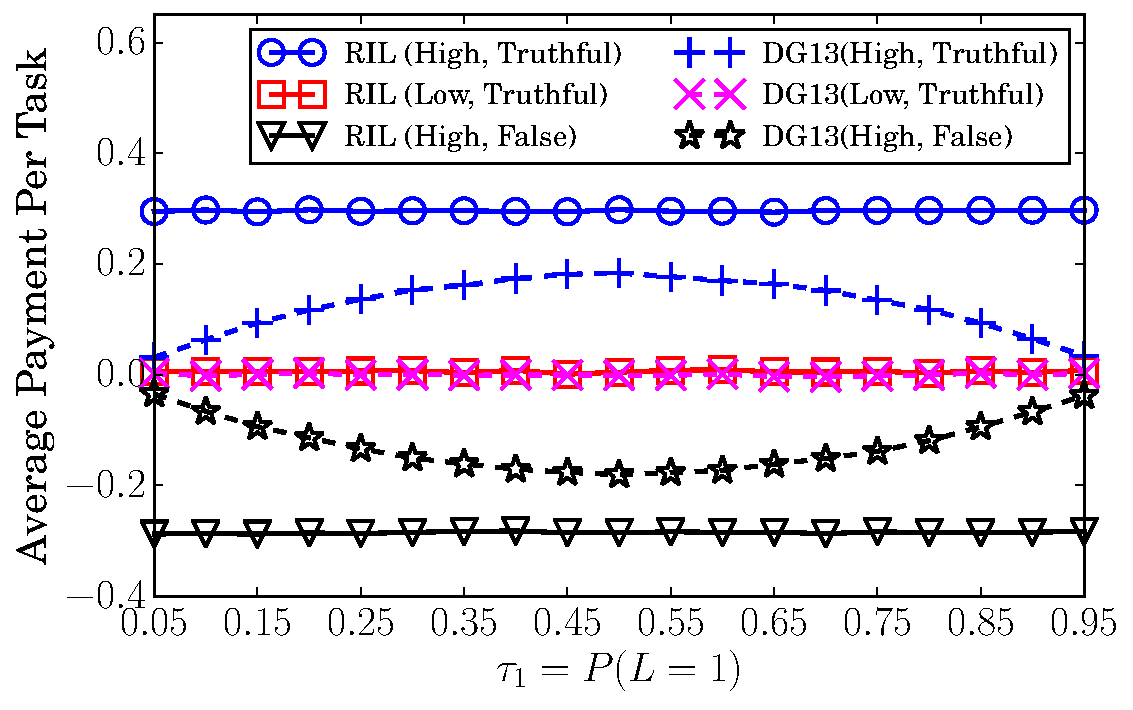
\includegraphics[width=\textwidth]{image/BPP1}
        \caption{\label{BIM2}}
    \end{subfigure}%
    ~
    \begin{subfigure}[t]{0.24\textwidth}
        \centering
        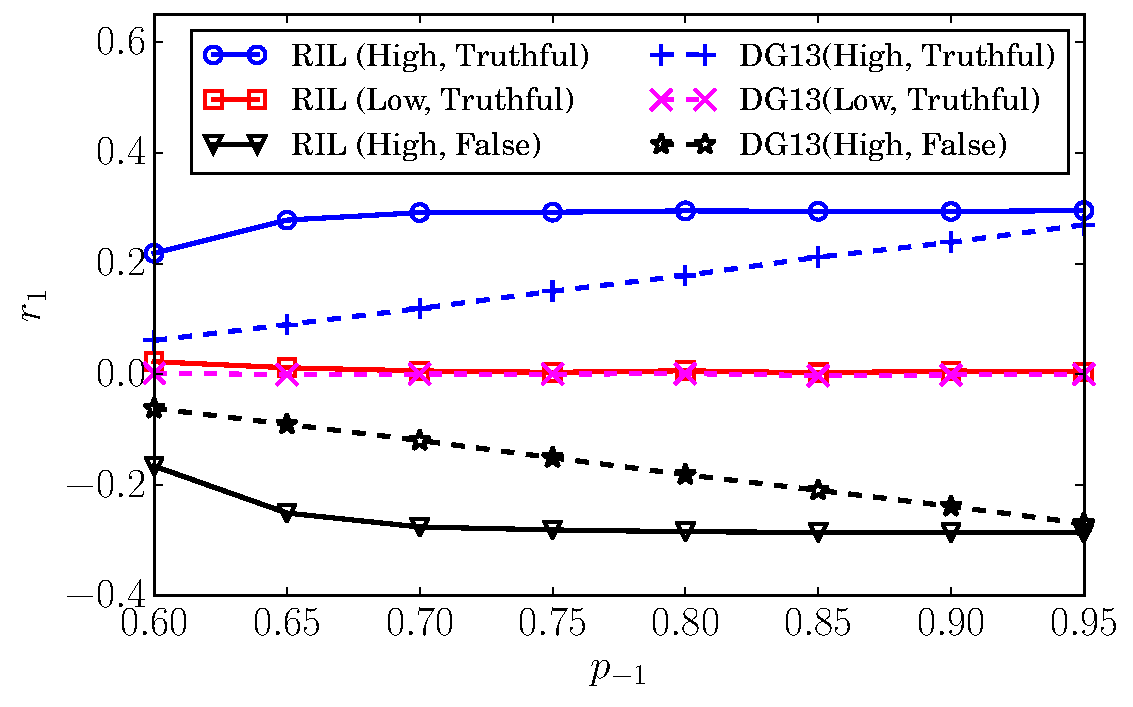
\includegraphics[width=\textwidth]{image/BPP2}
        \caption{\label{BIM3}}
    \end{subfigure}
        ~
    \begin{subfigure}[t]{0.24\textwidth}
        \centering
        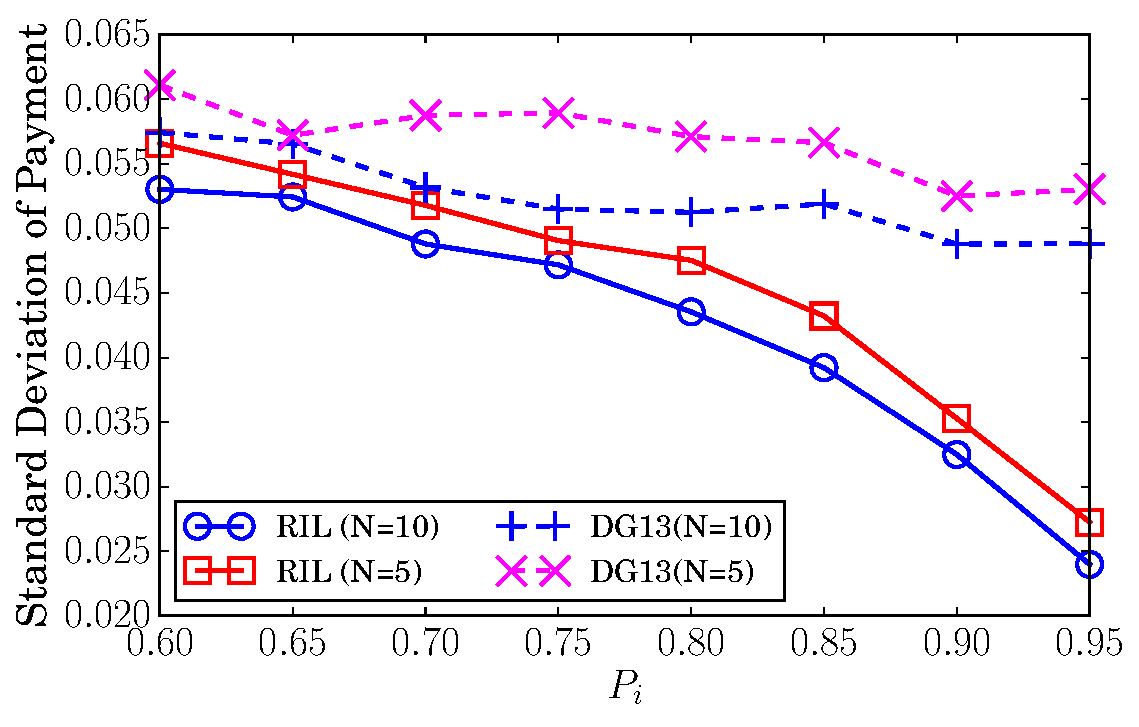
\includegraphics[width=\textwidth]{image/BPP3}
        \caption{\label{BIM4}}
    \end{subfigure}
	~
	\begin{subfigure}[t]{0.24\textwidth}
        \centering
        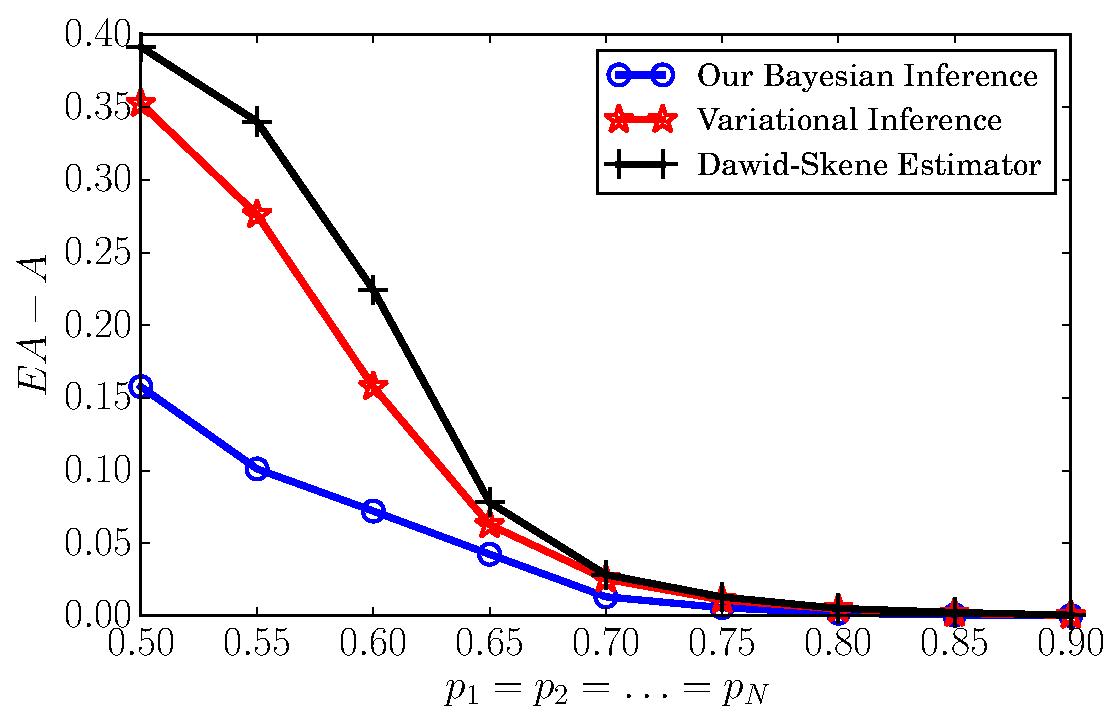
\includegraphics[width=\textwidth]{image/EXPC1}
        \caption{\label{BIM1}}
    \end{subfigure}
    \vspace*{-3mm}
    \caption{\label{BIM}One-step performance of our reinforcement incentive mechanism (RIM) (a) payment variation with the distribution of true labels (c) payment variation as the PoBC of other workers (d) the standard variance of the payment (d) the inference bias on label accuracy}
\end{figure*}

\section{Empirical Experiments}
In this section, we firstly test the one-step performance of our incentive mechanism by comparing it with the state-of-the-art incentive mechanism.
Then, we show the advantages of including the reinforcement algorithm via conducting experiments on three representative worker models, including fully rational, bounded rational and self-learning agents.

\subsection{One-Step Peroformance Analysis}
In Figures~\ref{BIM}a-c, we compare the average payments per task for worker $1$ in our incentive mechanism with DG13, the state-of-the-art peer prediction mechanism for binary labels~\cite{dasgupta2013crowdsourced,liu2017sequential}.
In all these experiments, we fix the scaling factor $a^t=1$ and set $M=100$, $N=10$, $p_H=0.8$ and $b=0$.
The labels are generated by simulating workers' observation process.
We firstly generate the true label for task $j$ based on the true label distriubtion $(\tau_1, \tau_2)$.
Then, we generate worker $i$'s label for task $j$ based on worker $i$'s PoBC $p_i$ and the true label $L(j)$.
For each point in these figures, we run the experiments for $1000$ rounds and present the means.

In Figure~\ref{BIM}a and b, we show the variation of the payment for worker $1$ with the distribution of true labels and the strategies of other workers, respectively.
More specifically, in Figure~\ref{BIM2}, we let all the other workers report truthfully and exert high efforts ($p_{i\neq 1}=p_H$), and meanwhile increase $\tau_1$ from $0.05$ to $0.95$.
In Figure~\ref{BIM3}, we let $\tau_1=0.5$, and increase $p_{i\neq 1}$ from $0.6$ to $0.95$.
From these two figures, we can find that the payment for worker $1$ in our mechanism almost only depend on worker $1$'s own strategy.
By contrast, the payments in DG13 is severely affected by the distribution of true labels and the strategies of other workers.
Furthermore, in Figure~\ref{BIM4}, we present the standard variance of the payment for worker $1$.
We let $\tau_1=0.5$, $p_{i\neq 1}=p_H$ and meanwhile increase $p_1$ from $0.6$ to $0.95$.
Form the figure, we can find that the payment vairance of our mechanism is much smaller than that of DG13.
All in all, our mechanism is much fairer and more stable than DG13.
This is because we can fully exploit the information provided by all workers while traditional peer prediciton mechanisms only compare the labels of two workers. 


In Figure~\ref{BIM1}, we compare our Bayesian inference algorithm with two popular inference algorithms in the studies of crowdsourcing, that is, the Dawid-Skene estimator~\cite{dawid1979maximum,raykar2010learning} and the variational inference estimator~\cite{liu2012variational,chen2015statistical}.
Here, we set workers' PoBC $p_i$ to be equal and increase the value of $p_i$ from $0.5$ to $0.9$, which means the quality of labels is gradually improved.
The other settings are the same as Figure~\ref{BIM3}.
From the figure, we can find that, when the quality of labels is very low, the inference bias of the Dawid-Skene and variational inference estimators on the label accuracy can be larger than $0.3$ while the range of the label accuracy is only $[0.5,1.0]$.
This observation shows that these two estimators become over-optimistic for low-quality labels, which will be disastrous for our reinforcement algorithm.
Thus, we develop a novel Bayesian inference algorithm which reduces the inference bias for low-quality labels by considering the connection between tasks.



%In the literature of crowdsourcing, the Dawid-Skene estimator is the most popular method used to infer the true labels~\cite{dawid1979maximum,raykar2010learning}.
%The variational inference estimator, which has the similar Bayesian model to our inference algorithm, is also widely-adopted in the existing studies of crowdsourcing~\cite{liu2012variational,chen2015statistical}.
%To compare different estimators, we set $M=100$ and $N=10$ in Figure~\ref{BIM1}. Also, we let the score of all workers be equal, namely $p_1= \ldots=p_N$, and increase the value of $p_i$ from $0.5$ to $0.9$. Meanwhile, we set the true label distribution as the uniform distribution, namely $\tau_1=\tau_2=0.5$. For a given $p_i$, we firstly generate the true labels and then the labels of all workers both by the Bernoulli distribution. For each value of $p_i$, we run the experiments for $1000$ rounds. To show the bias of inference, we calculate the average value differences between the posterior expected accuracy $\mathbb{E}A$ and the real accuracy $A$. From the figure, we can find that, when workers can provide not-so-bad labels ($p_i>0.75$), both the two above estimators and our inference algorithm have very small bias, which agrees with the good performance of these estimators in the literature~\cite{raykar2010learning,liu2012variational}. However, if workers can only provide low-quality labels, the bias of the Dawid-Skene and variational inference estimators will become unacceptable, because the difference can be larger than $0.3$ while both $\mathbb{E}A$ and $A$ belong to $[0.5,1.0]$. In this case, we cannot use $\mathbb{E}A$ to calculate the utility of the data requester as Equation~\ref{utility}. By contrast, the bias of our Bayesian inference algorithm is much smaller, which is the foundation of our reinforcement incentive mechanism.
%
%
%In Figures~\ref{BIM}b-d, we focus on $r_1$, namely, the per-task-reward received by worker $1$. Here, DG13~\cite{dasgupta2013crowdsourced,liu2017sequential}, which is the state-of-the-art incentive mechanism for binary labels, is employed as the benchmark.
%DG13 decides the reward for a worker by comparing his labels with the labels provided by another randomly selected worker.
%By elaborately designing the reward rules, it can also ensure reporting truthfully and exert high efforts to be a Nash equilibrium for all workers.
%In all these experiments, we set $p_H=0.8$, $p_L=0.5$, and keep the other settings the same as those in Figure~\ref{BIM1}.
%
%In Figure~\ref{BIM2}, we let $p_{-1}=p_H$, where the subscript $-1$ denotes all the workers except for worker $1$.
%We change the distribution of true labels by increasing $\tau_1$ from $0.05$ to $0.95$ and compare the average values of $r_1$ corresponding to the different strategies of worker $1$.
%In Figure~\ref{BIM3}, we fix the distribution of true labels to be the uniform distribution, namely, $\tau_1=\tau_2=0.5$, and increase $p_{-1}$ from $0.6$ to $0.95$.
%From these two figures, we can find that the rewards provided by our mechanism are almost not affected by the variation of the distribution of true labels and the strategies of the other workers.
%This observation reveals that $\mathbb{E}\tilde{p}_1$ converges to $p_1$ in most cases.
%The only exception is $p_{-1}<0.7$ in Figure~\ref{BIM3} where the low-quality labels will lead to a remarkable bias of inference.
%Even in this case, worker $1$ can only get the maximal reward when $p_1=p_H$, which shows the attracting ability of our mechanism to induce truthful reports and high efforts.
%By contrast, $r_1$ in DG13 is severely affected by the distribution of true labels and the strategies of other workers.
%For example, in Figure~\ref{BIM3}, if the other workers lower their efforts, the reward received by worker $1$ will also decrease, although worker $1$ never changes his strategies.
%Thereby, for worker $1$, our Bayesian incentive mechanism is much fairer than DG13.
%
%In Figure~\ref{BIM4}, we set $\tau_1=\tau_2=0.5$ and $p_{-1}=p_H$. We change worker $1$'s strategies by increasing $p_1$ from $0.6$ to $0.95$. Under these settings, the average values of $r_1$ corresponding to our mechanism and DG13 both can reflect the variation of $p_1$ very well. Thus, we focus on the standard variance comparison of $r_i$ in Figure~\ref{BIM4}.
%If the variance is very large, the reward received by worker $1$ when $p_1=p_H$ may become lower than the reward when $p_1<p_H$.
%If this case happens, it will significantly discourage worker $1$.
%For example, in Figure~\ref{BIM2}, when $\tau_1=0.05$, for DG13, the difference between $r_1(p_1=p_H)$ and $r_1(p_1=0.5)$ is around $0.06$.
%On the other hand, from Figure~\ref{BIM4}, the standard variance of $r_1$ is around $0.052$, which means there is a quite high probability for $r_1(p_1=p_H)<r_1(p_1=0.5)$.
%From Figure~\ref{BIM4}, we can find that our Bayesian incentive mechanism has a lower variance than DG13.
%If we take the fairness of our mechanism into consideration, we can conclude that our mechanism is more stable than DG13 in inducing truthful reports and high efforts from workers.


%\begin{equation}
%P(L(j)=1)=\tau_1{\prod}_{k\neq i}p_H^{\delta_{kj1}}(1-p_H)^{\delta_{kj2}}
%\end{equation}
%where $\lambda_0=\log(\tau_1/\tau_2)$ and $\lambda_i=\log(p_i/\bar{p}_i)$. For worker $i$, we assume that all other workers report truthfully and exert high efforts. Suppose the real true label is $1$. In order to ensure $\mathbb{E}[m/M]$ to approach $0$, the probability ratio in Equation~\ref{Ratio} must be positive with almost $1.0$ probability. Thus, we can directly discard the absolute operation in Equation~\ref{vot} and calculate the expected value of task $j$ as
%\begin{equation}
%\mathbb{E}_1v(j)\approx \lambda_0+(N-1)(2p_H-1)\lambda_H+(2p_i-1)\lambda_i.
%\end{equation}
%Similarly, if the real true label is $2$, then
%\begin{equation}
%\mathbb{E}_2v(j)\approx -\lambda_0+(N-1)(2p_H-1)\lambda_H+(2p_i-1)\lambda_i.
%\end{equation}
%Thus, the average task value $v$ satisfies
%\begin{equation}
%\begin{split}
%&\mathbb{E}v = \tau_1 \mathbb{E}_1v(j) + \tau_2\mathbb{E}_2v(j)\\
%&=(2\tau_1-1)\lambda_0+(N-1)(2p_H-1)\lambda_H+(2p_i-1)\lambda_i.
%\end{split}
%\end{equation}
%
%Suppose the true label is $1$.
%\begin{equation}
%x= \log\frac{P(L=1)}{P(L=2)}=g+\sum_{i=1}^{N}f(x_i,y_i,w_i,z_i)
%\end{equation}
%\noindent where $g=g_1-g_2$, and 
%\begin{equation*}
%g_1=\log(s_1+t_2+1)\;,\;g_2=\log(s_2+t_1+1).
%\end{equation*}
%Omitting the subscript in $f$, we can have $f=f_1-f_2$ with probability $p$ and $f=f_2-f_1$ with probability $1-p$. Here,
%\begin{equation*}
%f_1=\log(x+z+2)\;,\;f_2=\log(w+y+1).
%\end{equation*}
%Thus, we can have
%\begin{equation}
%\mathbb{E}g = \mathbb{E}g_1-\mathbb{E}g_2 \;,\;
%\mathbb{E}f = (2p-1)(\mathbb{E}f_1-\mathbb{E}f_2).
%\end{equation}
%From the previous proof, we know that $P(m)$ is very small when $m>>1$. Thus, we mainly focus on the region where $m$ is relatively small. For a given small $m$,
%\begin{equation}
%\mathbb{E}_{s_1, t_2}g_1\approx \mathbb{E}_{t_2}\log(np+t_2+1)
%\end{equation}
%\begin{equation}
%\log(np+t_2+1) = \log(np+1)+\sum_{i=1}^{\infty}(-1)^{i-1}q^i
%\end{equation}
%\begin{equation}
%q = \frac{t_2}{np+1}\Rightarrow 0\leq q^{i} \leq c^{i}\cdot \left(\frac{m}{M}\right)^i\leq c^{i}\frac{m}{M}
%\end{equation}
%Then,
%\begin{equation}
%\mathbb{E}g_1 \approx \mathbb{E}_{m}\log(1+Mp-mp)
%\end{equation}
%\begin{equation}
%\log(1+Mp-mp)\approx\log(1+Mp)+\sum_{i=1}^{\infty}(-1)^{i}\left(\frac{m}{M}\right)^i
%\end{equation}
%Using the similar way of approximation for the computation of $\mathbb{E}g_2$, $\mathbb{E}f_1$ and $\mathbb{E}f_2$, we can have
%\begin{equation}
%\begin{split}
%\mathbb{E}g_1\approx \log(Mp)\;,\;\mathbb{E}g_2\approx \log(M(1-p))\\
%\mathbb{E}f_1\approx \log(Mp)\;,\;\mathbb{E}f_2\approx \log(M(1-p))
%\end{split}
%\end{equation}
%Thus, if all workers exert high efforts and report truthfully,
%\begin{equation}
%    \mathbb{E}x \approx \log\lambda_0 + {\sum}_{i=1}^{N}\log\lambda_{i,H}
%\end{equation}
%If the true label is $2$, then
%\begin{equation}
%    \mathbb{E}x \approx \log\lambda_0 - {\sum}_{i=1}^{N}\log\lambda_{i,H}
%\end{equation}
%Thereby,
%\begin{equation}
%    \mathbb{E}|x|\approx (2p_0-1)\log\lambda_0+ {\sum}_{i=1}^{N}\log\lambda_{i,H}
%\end{equation}
%When, for example, worker $1$ deviate from the desired equilibrium strategy, the non-equilibrium state correspond to
%\begin{equation}
%    \mathbb{E}|x'|\approx (2p_0-1)\log\lambda_0+ \log\lambda_{1}+{\sum}_{i=2}^{N}\log\lambda_{i,H}
%\end{equation}
%The minimal value of $\mathbb{E}|x'|$ is reached when worker $1$ exert high efforts and report falsely, namely $\log\lambda_{i}=-\log\lambda_{i,H}$.
%Thus, the maximal reward increment brought by worker $1$'s strategy switch is
%\begin{equation}
%    V_1 = F(\mathbb{E}x)-F(\mathbb{E}x') \approx 2\log\lambda_{1,H}\cdot \left.\frac{\mathrm{d}F}{\mathrm{d}x}\right|_{x=x_H}
%\end{equation}
%Since $p_0$ is difficult to estimate, we define the upper bound of the value increment as
%\begin{equation}
%    V = 2\max_{i}\log\lambda_{i,H} \cdot  \max_{x\in [x_H, \infty)}\frac{\mathrm{d}F}{\mathrm{d}x} 
%\end{equation}
%where $x_H= \log\lambda_0 + {\sum}_{i=1}^{N}\log\lambda_{i,H}$.
%Considering the discounted reward calculation in reinforcement learning, we can know the maximum value difference can be created by the manipulation of any worker is $(1-\rho)^{-1}V$. Meanwhile, if the reinforcement part increases the scaling factor by $\delta$ to obtain the reward increment, we need to pay more than $\sum_{i=1}^{N}M\delta (p_{i,H}-0.5)$. Thus, if we want to prevent the reinforcement learning module from the adversarial manipulation, the minimal gap $\delta$ between to two available scaling factors should satisfy
%\begin{equation}
%    \sum_{i=1}^{N}M\delta (p_{i,H}-0.5) > V.
%\end{equation}

\section{Future Work and Conclusion}
In this paper, we build a novel sequential data acquisition mechanism for crowdsourcing.
In each time step, our mechanism uses a Bayesian inference algorithm to , and our payments to workers are proportional to these estimates.
We adjust the scaling factor of the payments by developing a RL algorithm which can learn how workers respond to the payments in the background.
We theoretically prove that our mechanism is incentive compatible.
We also empirically show that our Bayesian inference algorithm can help to improve the robustness and lower the variance of payments.
Meanwhile, our RL algorithm can adapt our mechanism to different kinds of worker models and thus consistently improve the utility of the data requester.
In the future, we will firstly extend our proof in Section 5 to more general cases where $m_i^t<M$.
Secondly, for more practical cases where the number of workers is very large and the mapping between workers and tasks is very sparse, we will improve our RL algrithm by involving more complex state representations.

\bibliographystyle{icml2018}
\bibliography{ref}

\end{document}



